\documentclass[12pt, a4paper]{article}

% ── Packages ─────────────────────────────────────────────────────────────────
\usepackage[utf8]{inputenc}
\usepackage[T1]{fontenc}
\usepackage[portuguese]{babel}
\usepackage{geometry}
\usepackage{graphicx}
\usepackage{booktabs}
\usepackage{array}
\usepackage{longtable}
\usepackage{hyperref}
\usepackage{amsmath}
\usepackage{amssymb}
\usepackage{listings}
\usepackage{xcolor}
\usepackage{float}
\usepackage{caption}
\usepackage{subcaption}
\usepackage{parskip}
\usepackage{setspace}
\usepackage{fancyhdr}
\usepackage{titlesec}
\usepackage{enumitem}
\usepackage{multirow}

% ── Macros e utilitários ─────────────────────────────────────────────────────
\newcommand{\acirc}{A}
\newcommand{\eref}[1]{(\ref{#1})}

% ── Geometria ────────────────────────────────────────────────────────────────
\geometry{
    top=2.5cm, bottom=2.5cm,
    left=2.5cm, right=2.5cm
}

% ── Cores e listings ─────────────────────────────────────────────────────────
\definecolor{codebg}{rgb}{0.97,0.97,0.97}
\definecolor{codeframe}{rgb}{0.8,0.8,0.8}
\definecolor{keyword}{rgb}{0.13,0.29,0.53}
\definecolor{comment}{rgb}{0.4,0.4,0.4}
\definecolor{string}{rgb}{0.13,0.53,0.13}

\lstset{
    language=Python,
    backgroundcolor=\color{codebg},
    frame=single,
    rulecolor=\color{codeframe},
    basicstyle=\ttfamily\footnotesize,
    keywordstyle=\color{keyword}\bfseries,
    commentstyle=\color{comment}\itshape,
    stringstyle=\color{string},
    breaklines=true,
    breakatwhitespace=true,
    numbers=left,
    numberstyle=\tiny\color{comment},
    numbersep=5pt,
    showstringspaces=false,
    tabsize=4,
    captionpos=b,
}

% ── Hyperref ─────────────────────────────────────────────────────────────────
\hypersetup{
    colorlinks=true,
    linkcolor=blue!60!black,
    urlcolor=blue!60!black,
    citecolor=blue!60!black,
    pdftitle={Previsão Probabilística de Futebol - Versão Jupyter Notebook},
    pdfauthor={Duarte Prazeres},
}

% ── Cabeçalho / rodapé ───────────────────────────────────────────────────────
\pagestyle{fancy}
\fancyhf{}
\rhead{\small Inteligência Artificial Probabilística}
\lhead{\small Duarte Prazeres}
\rfoot{\thepage}
\renewcommand{\headrulewidth}{0.4pt}

% ── Título ───────────────────────────────────────────────────────────────────
\title{
    \vspace{-1cm}

    {\large Inteligência Artificial Probabilística 2025/2026}\\[0.2cm]

    \rule{\linewidth}{0.5pt}\\[0.4cm]
    {\LARGE \textbf{Previsão Probabilística de Resultados de Futebol}}\\[0.3cm]
    {\large Projeto Final -- Versão Jupyter Notebook}\\[0.2cm]
    \rule{\linewidth}{0.5pt}
}

\author{
    Duarte Prazeres, 2023214962 \\
    \small
}

%\date{\today}

% ═════════════════════════════════════════════════════════════════════════════
\begin{document}
% ═════════════════════════════════════════════════════════════════════════════

\maketitle
\thispagestyle{empty}

% ── Resumo ───────────────────────────────────────────────────────────────────
\begin{abstract}
Este relatório descreve o desenvolvimento de um sistema de previsão probabilística para resultados de jogos da Liga de Futebol Portuguesa, elaborado como projeto final da unidade curricular de \emph{Introdução à Inteligência Artificial Probabilística} (IAP).

O projeto está organizado em quatro partes:

\begin{enumerate}[leftmargin=2em]
  \item \textbf{Parte 0 — Pipeline de Dados e EDA:} Construção de um \textit{dataset} a partir de dados históricos da liga portuguesa (2006--2026), incluindo limpeza, engenharia de \textit{features} e análise exploratória.
  \item \textbf{Parte 1 — Redes Bayesianas:} Modelação probabilística através de \textit{knowledge engineering} (KE) e aprendizagem de estrutura automática (\textit{Hill-Climbing}), com inferência por propagação de crenças.
  \item \textbf{Parte 2 — Classificação Probabilística e Incerteza:} Treino e avaliação de classificadores Naive Bayes (Gaussiano e Categórico), \textit{Conformal Prediction}, calibração e otimização Bayesiana de hiperparâmetros.
  \item \textbf{Parte 3 — Teoria de Utilidade e Decisão:} Comparação de estratégias de decisão (modelo puro vs.\ \textit{reject option}) recorrendo a probabilidades implícitas das \textit{odds} de apostas.
\end{enumerate}

Os resultados demonstram que modelos probabilísticos estruturados fornecem estimativas de incerteza credíveis e que a integração de informação de mercado pode melhorar a tomada de decisão.
\end{abstract}

\newpage
\tableofcontents
\newpage

% ═════════════════════════════════════════════════════════════════════════════
\section{Organização do Projeto em Jupyter Notebooks}
% ═════════════════════════════════════════════════════════════════════════════

\subsection{Estrutura do Projeto}

Este projeto foi desenvolvido utilizando \textbf{Jupyter Notebooks}, uma plataforma interativa que combina código executável, visualizações \textit{inline} e documentação em Markdown num único ambiente integrado. Esta abordagem é ideal para exploração de dados, prototipagem rápida e comunicação de resultados.

O projeto está organizado em \textbf{quatro notebooks sequenciais}, cada um correspondendo a uma parte do projeto:

\begin{enumerate}
  \item \texttt{Part0\_Data\_Pipeline.ipynb} -- Pipeline de dados e análise exploratória
  \item \texttt{Part1\_Bayesian\_Networks.ipynb} -- Redes Bayesianas e inferência
  \item \texttt{Part2\_Classification\_Uncertainty.ipynb} -- Classificação probabilística
  \item \texttt{Part3\_Utility\_Decision.ipynb} -- Teoria de utilidade e decisão
\end{enumerate}

\subsection{Como Executar os Notebooks}

Os notebooks devem ser executados \textbf{sequencialmente}, pois cada um depende dos dados e resultados gerados pelos anteriores. Para executar o projeto:

\begin{enumerate}
  \item \textbf{Instalar dependências:}
  \begin{lstlisting}[language=bash]
pip install -r requirements.txt
  \end{lstlisting}

  \item \textbf{Iniciar Jupyter Notebook:}
  \begin{lstlisting}[language=bash]
cd notebook/
jupyter notebook
  \end{lstlisting}

  \item \textbf{Executar os notebooks na ordem:}
  \begin{itemize}
    \item Abrir \texttt{Part0\_Data\_Pipeline.ipynb} e executar todas as células (\texttt{Cell > Run All})
    \item Repetir o processo para \texttt{Part1}, \texttt{Part2} e \texttt{Part3}
  \end{itemize}
\end{enumerate}

\subsection{Benefícios da Abordagem Jupyter Notebook}

A organização do projeto em Jupyter Notebooks oferece vantagens significativas para análise de dados e comunicação de resultados científicos. A \textbf{interatividade} é o benefício central desta abordagem -- permite executar código célula a célula, facilitando a experimentação incremental e depuração imediata de problemas, algo impossível em scripts tradicionais onde é necessário executar tudo de uma vez.

As \textbf{visualizações \textit{inline}} melhoram dramaticamente a compreensão dos dados: gráficos, tabelas e figuras aparecem diretamente no notebook, ao lado do código que os gerou, criando uma conexão visual imediata entre análise e resultados. Esta proximidade elimina a necessidade de alternar entre ficheiros e facilita a interpretação.

A \textbf{documentação integrada} através de células Markdown permite adicionar explicações textuais, equações matemáticas (em LaTeX) e contexto diretamente no fluxo da análise. Isto transforma o notebook numa narrativa completa que combina código, resultados e interpretação num único documento coerente. Esta \textbf{narrativa linear} sequencial facilita contar uma história dos dados aos resultados finais, guiando o leitor através do raciocínio analítico de forma natural e pedagógica.

A \textbf{reprodutibilidade} é garantida pela natureza autodocumentada dos notebooks: todos os passos da análise -- desde o carregamento de dados até às conclusões -- estão explicitamente registados e podem ser reexecutados para validar os resultados. Por fim, a abordagem é ideal para \textbf{exploração iterativa} e prototipagem rápida, permitindo testar hipóteses, ajustar parâmetros e visualizar resultados de forma ágil, características essenciais para análise exploratória de dados (EDA) e desenvolvimento de modelos.

\subsection{Estrutura de Ficheiros}

\begin{verbatim}
IAPproject/
  - compilar_relatorios.sh     # Script de compilacao dos relatorios
  - README.md
  - dataset/                   # Dataset partilhado por ambas as versoes
      - dataset.csv
  - notebook/
      - Part0_Data_Pipeline.ipynb
      - Part1_Bayesian_Networks.ipynb
      - Part2_Classification_Uncertainty.ipynb
      - Part3_Utility_Decision.ipynb
      - data/                    # Dados processados
          - requirements.txt
      - plots/                   # Graficos gerados
          - p0_*.png
          - p1_*.png
          - p2_*.png
          - p3_*.png
      - docs/                    # Este relatorio
          - relatorio_notebook.tex
          - relatorio_notebook.pdf
\end{verbatim}

% ═════════════════════════════════════════════════════════════════════════════
\section{Parte 0 --- Pipeline de Dados e Análise Exploratória}
% ═════════════════════════════════════════════════════════════════════════════

\subsection{Motivação e Origem dos Dados}

O conjunto de dados foi construído a partir dos resultados historicos da Liga Portuguesa de Futebol, abrangendo épocas de \textbf{2006 a 2026}. Os dados brutos incluem resultados (golos marcados e sofridos), \textit{odds} de casas de apostas (H/D/A), histórico de confrontos diretos (\textit{head-to-head}) e estatísticas de forma recente de cada equipa.

\subsection{Limpeza e Feature Engineering}

A pipeline de dados realiza as seguintes operações:

\subsubsection{Variáveis de forma recente}

Para cada jogo, são calculadas janelas de forma dos últimos 5 jogos:

\begin{itemize}
  \item \texttt{ht\_form\_points} / \texttt{at\_form\_points} — Pontos acumulados pelos últimos 5 jogos (casa/visitante).
  \item \texttt{ht\_form\_goals\_scored} / \texttt{at\_form\_goals\_scored} — Golos marcados nos últimos 5 jogos.
  \item \texttt{ht\_form\_goals\_conceded} / \texttt{at\_form\_goals\_conceded} — Golos sofridos nos últimos 5 jogos.
  \item \texttt{ht\_form\_wins} / \texttt{at\_form\_wins} — Vitórias nos últimos 5 jogos.
  \item \texttt{ht\_home\_form\_points} / \texttt{at\_away\_form\_points} — Forma específica em casa/fora.
\end{itemize}

\subsubsection{Variáveis de confronto direto (H2H)}

\begin{itemize}
  \item \texttt{h2h\_home\_wins}, \texttt{h2h\_draws}, \texttt{h2h\_away\_wins} — Contagem dos últimos encontros diretos.
  \item \texttt{h2h\_dominance} — Variável categórica: \texttt{Home}, \texttt{Away} ou \texttt{Even}.
\end{itemize}

\subsubsection{Discretizações categóricas}

\begin{itemize}
  \item \texttt{ht\_form} / \texttt{at\_form} — Forma geral categorizada em \textit{Excellent}, \textit{Good}, \textit{Average}, \textit{Poor}.
  \item \texttt{ht\_attack} / \texttt{at\_attack} — Capacidade ofensiva em \textit{Strong}, \textit{Average}, \textit{Weak}.
  \item \texttt{joint\_attack} — Concatenação da capacidade ofensiva de casa e visitante (\texttt{ht\_attack} ao lado de \texttt{at\_attack}), capturando a dinâmica conjunta do ataque esperado no jogo.
  \item \texttt{odds\_favorite} — Favorito segundo o mercado de apostas (\texttt{H}, \texttt{D}, \texttt{A}).
\end{itemize}

\subsubsection{Variável alvo}

\[
  \texttt{result} \in \{H,\; D,\; A\}
\]
onde $H$ = vitória caseira, $D$ = empate, $A$ = vitória visitante.

\subsection{Análise Exploratória de Dados}

\subsubsection{Distribuição dos resultados}

\begin{figure}[H]
  \centering
  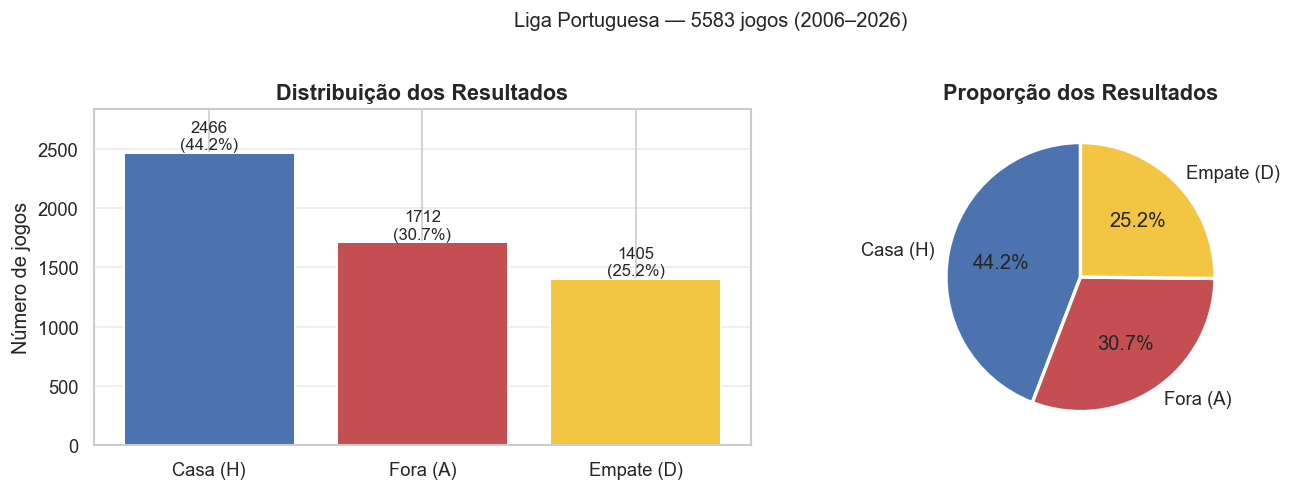
\includegraphics[width=0.65\textwidth]{../plots/p0_result_distribution.png}
  \caption{Distribuição dos resultados ao longo de todo o \textit{dataset}.}
  \label{fig:result_dist}
\end{figure}

Observa-se uma clara vantagem da equipa da casa: aproximadamente \textbf{44\%} de vitórias caseiras, \textbf{26\%} de empates e \textbf{30\%} de vitórias visitantes. Este desequilíbrio de classes é um fator relevante para a modelação, justificando o uso posterior de técnicas de reequilíbrio, como a aplicação de \textit{class weights} durante o treino dos classificadores para mitigar o viés estatístico face à classe minoritária (empate).

\subsubsection{Evolução temporal}

\begin{figure}[H]
  \centering
  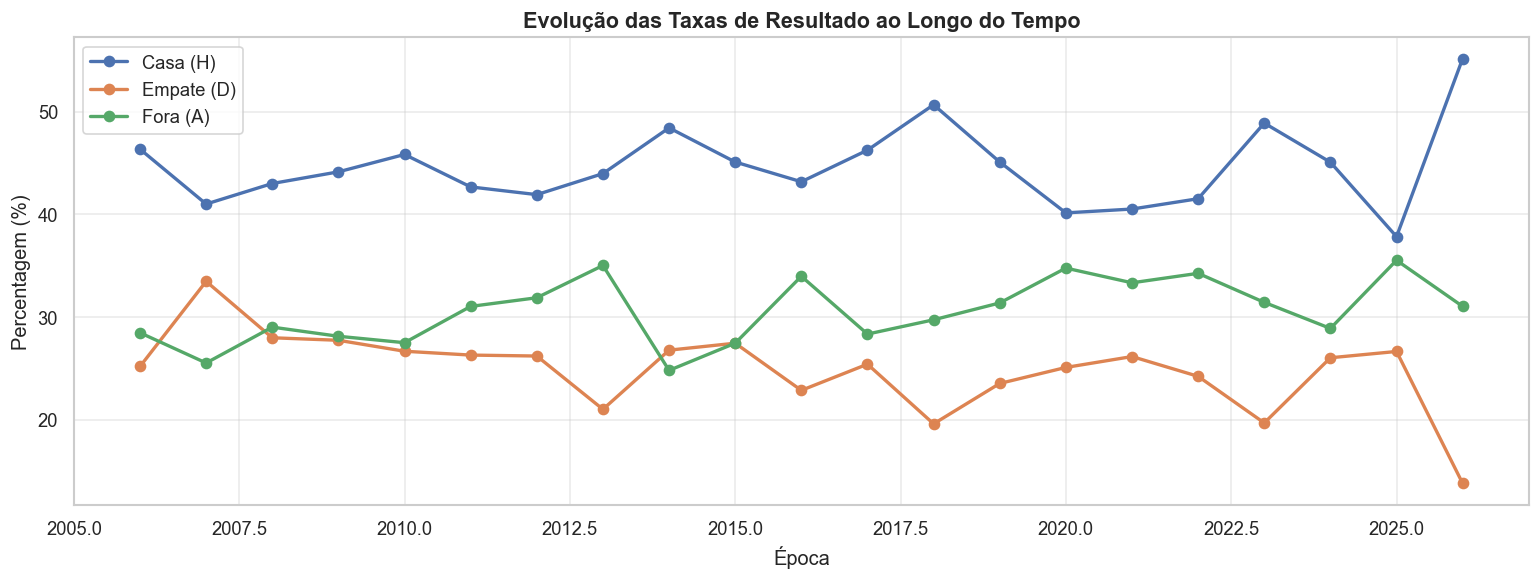
\includegraphics[width=\textwidth]{../plots/p0_results_over_time.png}
  \caption{Proporção de cada resultado ao longo dos anos.}
  \label{fig:results_time}
\end{figure}

A Figura~\ref{fig:results_time} revela que a vantagem caseira se mantém relativamente estável ao longo das épocas, embora com alguma variação sazonal.

\subsubsection{Forma recente vs.\ resultado}

\begin{figure}[H]
  \centering
  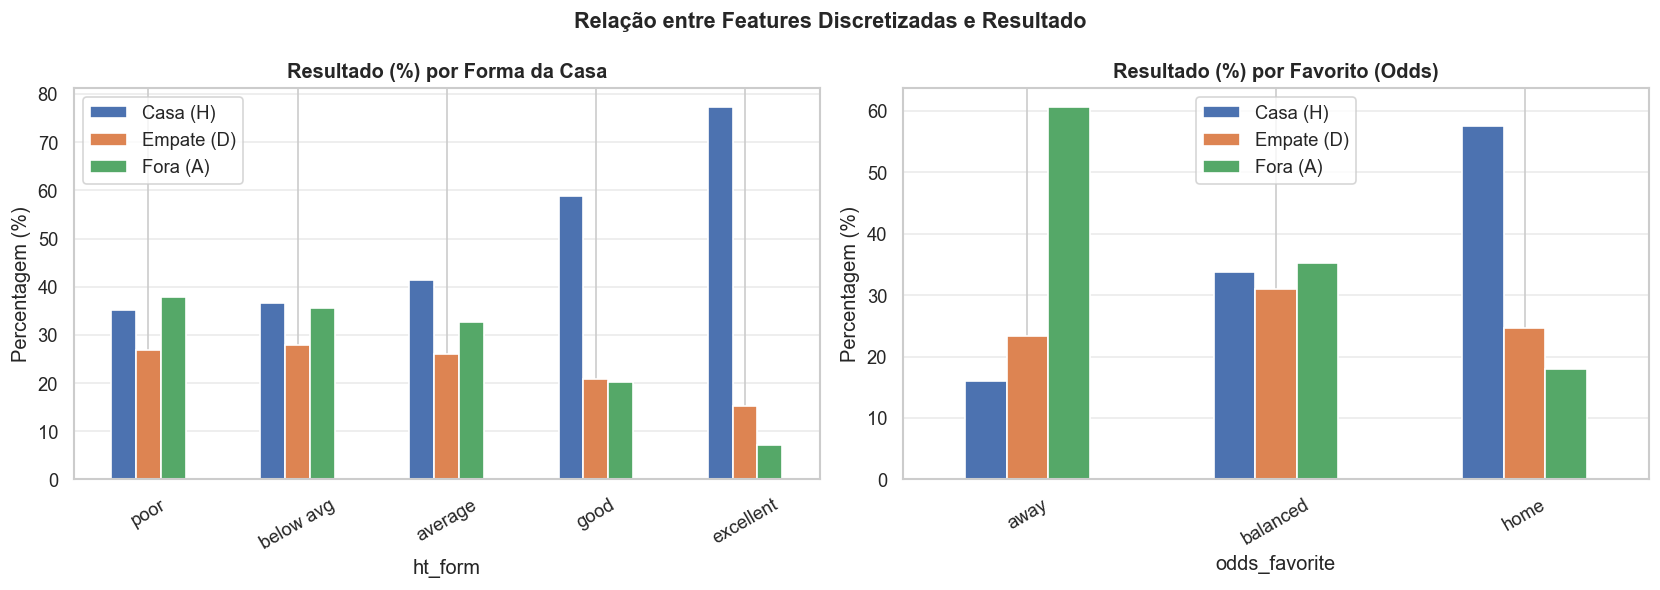
\includegraphics[width=\textwidth]{../plots/p0_form_vs_result.png}
  \caption{Relação entre a forma recente das equipas e o resultado do jogo.}
  \label{fig:form_result}
\end{figure}

Existe uma relação clara: equipas em melhor forma tendem a vencer mais. $p(\text{result}=H \mid \text{ht\_form}=\text{Excellent}) > p(\text{result}=H \mid \text{ht\_form}=\text{Poor})$.

\subsubsection{Matriz de correlação e distribuição de variáveis discretas}

\begin{figure}[H]
  \centering
  \begin{subfigure}[b]{0.48\textwidth}
    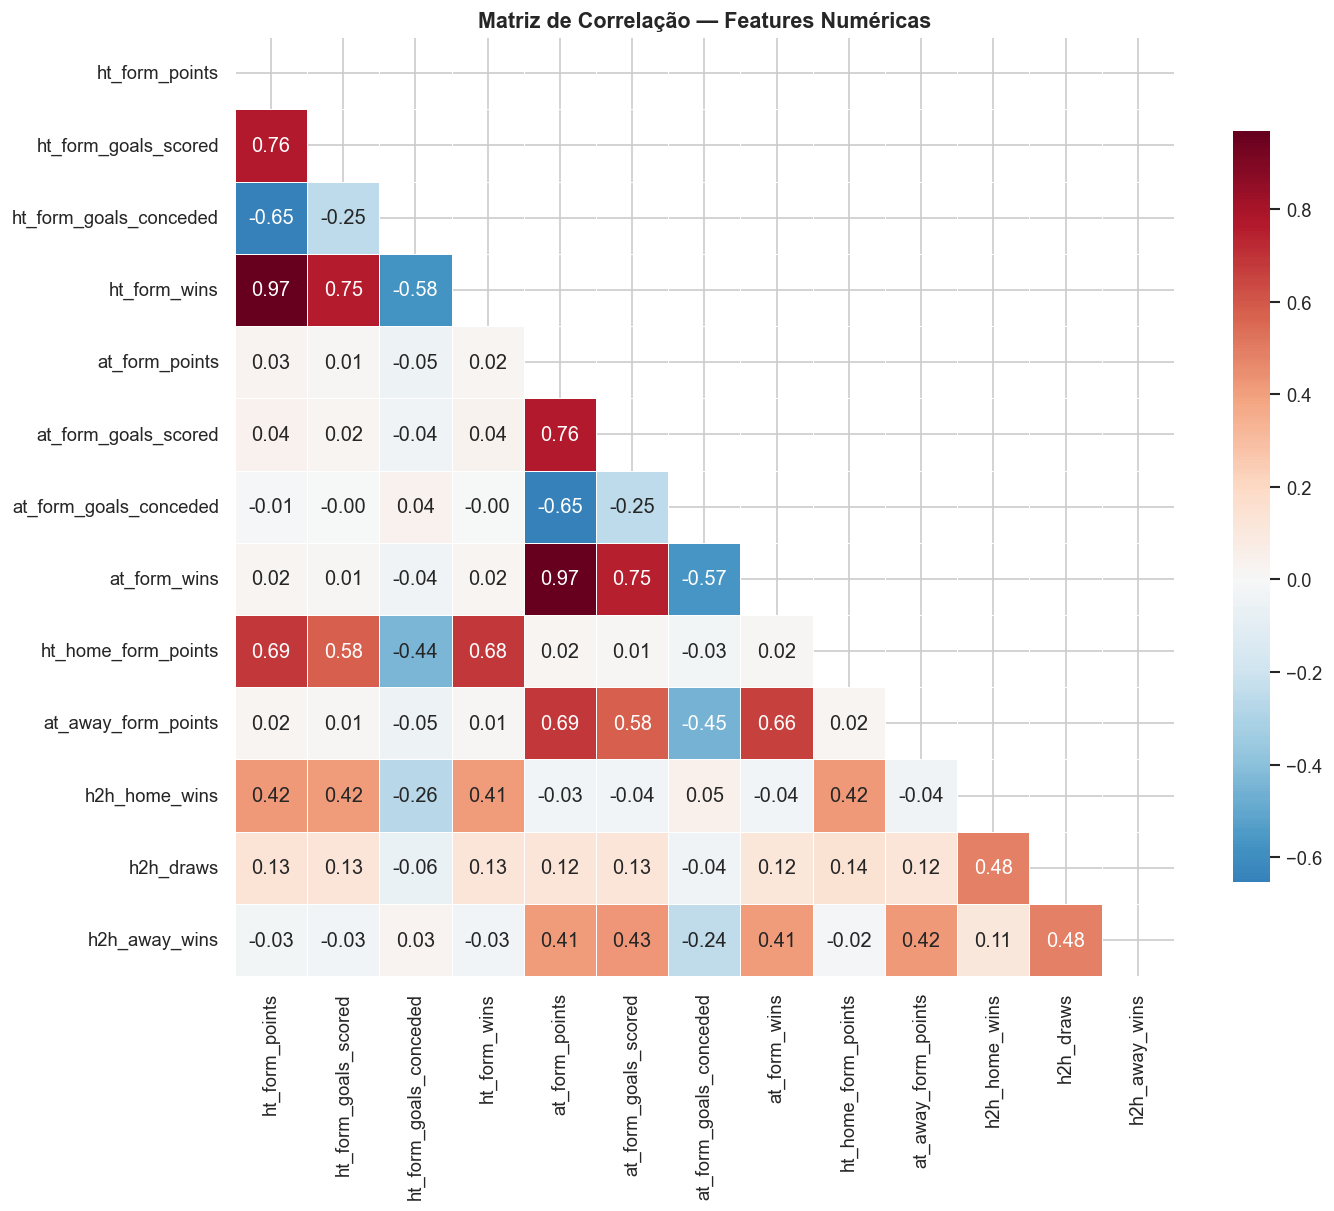
\includegraphics[width=\textwidth]{../plots/p0_correlation_matrix.png}
    \caption{Matriz de correlação das variáveis numéricas.}
    \label{fig:corr_matrix}
  \end{subfigure}
  \hfill
  \begin{subfigure}[b]{0.48\textwidth}
    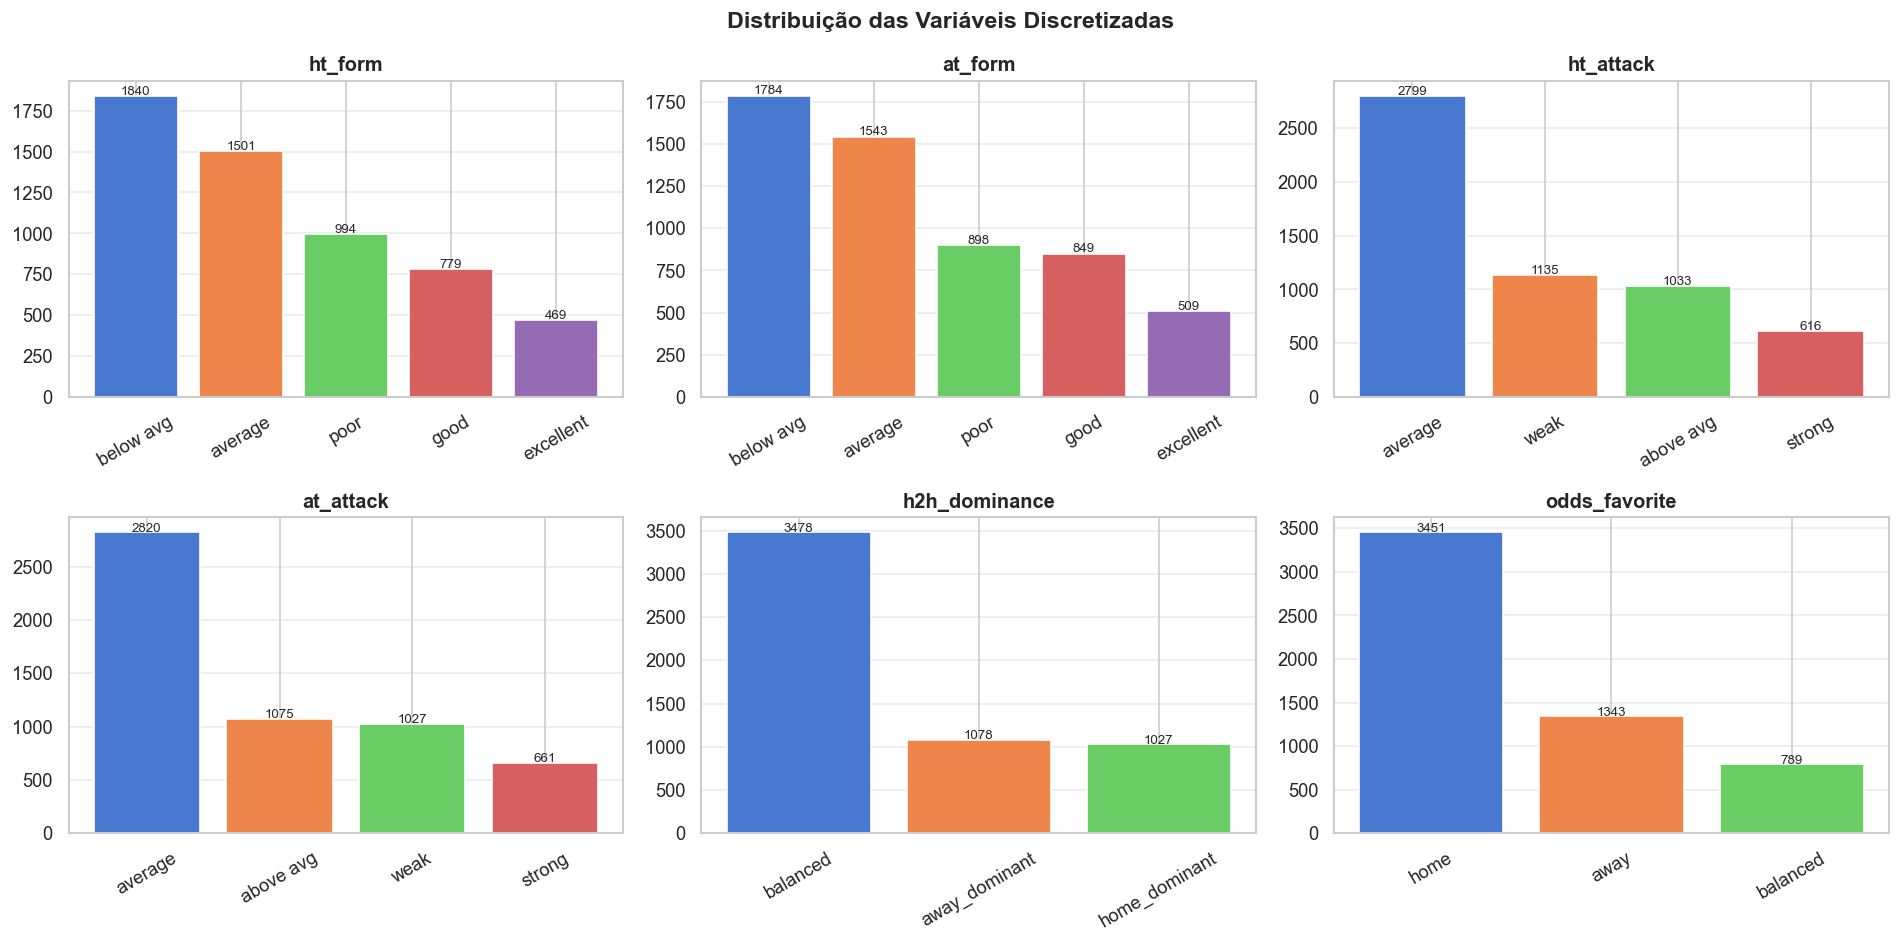
\includegraphics[width=\textwidth]{../plots/p0_discrete_vars.png}
    \caption{Distribuição das variáveis discretas.}
    \label{fig:discrete_vars}
  \end{subfigure}
  \caption{Análise das variáveis do \textit{dataset}.}
\end{figure}

A matriz de correlação (Figura~\ref{fig:corr_matrix}) mostra correlações positivas moderadas entre pontos de forma e golos marcados, e correlações negativas entre golos marcados e golos sofridos, confirmando a validade das \textit{features} construídas.

\subsection{Resumo do Dataset Final}

\begin{table}[H]
  \centering
  \caption{Estatísticas do \textit{dataset} final após limpeza.}
  \begin{tabular}{lcc}
    \toprule
    \textbf{Conjunto}  & \textbf{Período}         & \textbf{Jogos} \\
    \midrule
    Treino             & 2006-01-06 a 2021-12-30  & 4\,331         \\
    Teste              & 2022-01-02 a 2026-01-26  & 1\,252         \\
    \midrule
    \multicolumn{2}{l}{Total de \textit{features} (numéricas + categóricas)} & 21 \\
    \bottomrule
  \end{tabular}
  \label{tab:dataset}
\end{table}

\subsection{Divisão Temporal e Estratégias de Validação}

\subsubsection{Porquê Divisão Cronológica?}

A divisão entre treino e teste foi realizada de forma \textbf{cronológica} (e não aleatória) para evitar \textbf{\textit{data leakage}} em séries temporais. Se a divisão fosse aleatória, o modelo poderia ser treinado com dados do futuro e testado com dados do passado, inflacionando artificialmente os resultados.

Em previsão de futebol, o objetivo é prever jogos \textit{futuros} com base em informação \textit{passada}. A divisão temporal (treino: 2006--2021, teste: 2022--2026) respeita esta causalidade temporal, simulando um cenário realista de deploy do modelo.

\subsubsection{Conjuntos de Validação}

Embora não exista um conjunto de validação \textit{fixo} separado, foram utilizadas várias estratégias de validação interna ao longo do projeto:

\begin{table}[H]
  \centering
  \caption{Estratégias de validação utilizadas em cada parte do projeto.}
  \begin{tabular}{lp{8cm}}
    \toprule
    \textbf{Técnica} & \textbf{Estratégia de Validação} \\
    \midrule
    \textbf{Conformal Prediction} & Split interno: 80\% dos dados de treino para ajuste + 20\% para calibração do conjunto de previsão \\[0.3cm]
    \textbf{Calibração de Modelos} & Split interno (80\%/20\%) para calibração isotónica: ajustar modelo no primeiro split, calibrar no segundo \\[0.3cm]
    \textbf{Otimização Bayesiana} & \texttt{TimeSeriesSplit} com validação cruzada temporal (respeitando ordem cronológica) em 3 folds \\
    \bottomrule
  \end{tabular}
  \label{tab:validation}
\end{table}

Esta abordagem garante que todas as estimativas de incerteza e hiperparâmetros são ajustados sem contaminar o conjunto de teste final.

% ═════════════════════════════════════════════════════════════════════════════
\section{Parte 1 --- Redes Bayesianas}
% ═════════════════════════════════════════════════════════════════════════════

\subsection{Enquadramento Teórico}

Uma \textbf{Rede Bayesiana} (RB) é um modelo gráfico probabilístico que representa as dependências condicionais entre variáveis aleatórias através de um grafo dirigido acíclico (DAG). Formalmente:

\[
  P(X_1, X_2, \ldots, X_n) = \prod_{i=1}^{n} P(X_i \mid \text{pa}(X_i))
\]

onde $\text{pa}(X_i)$ denota o conjunto de nós pai de $X_i$ no DAG.

Neste projeto exploram-se duas abordagens para definir a estrutura da rede:
\begin{enumerate}
  \item \textbf{Knowledge Engineering (KE):} Estrutura definida manualmente com base no conhecimento de domínio.
  \item \textbf{Hill-Climbing:} Aprendizagem automática de estrutura por pesquisa local no espaço de DAGs.
\end{enumerate}

\subsection{Knowledge Engineering (KE)}

A rede de KE foi construída refletindo o conhecimento sobre como os resultados de futebol são influenciados:

\begin{figure}[H]
  \centering
  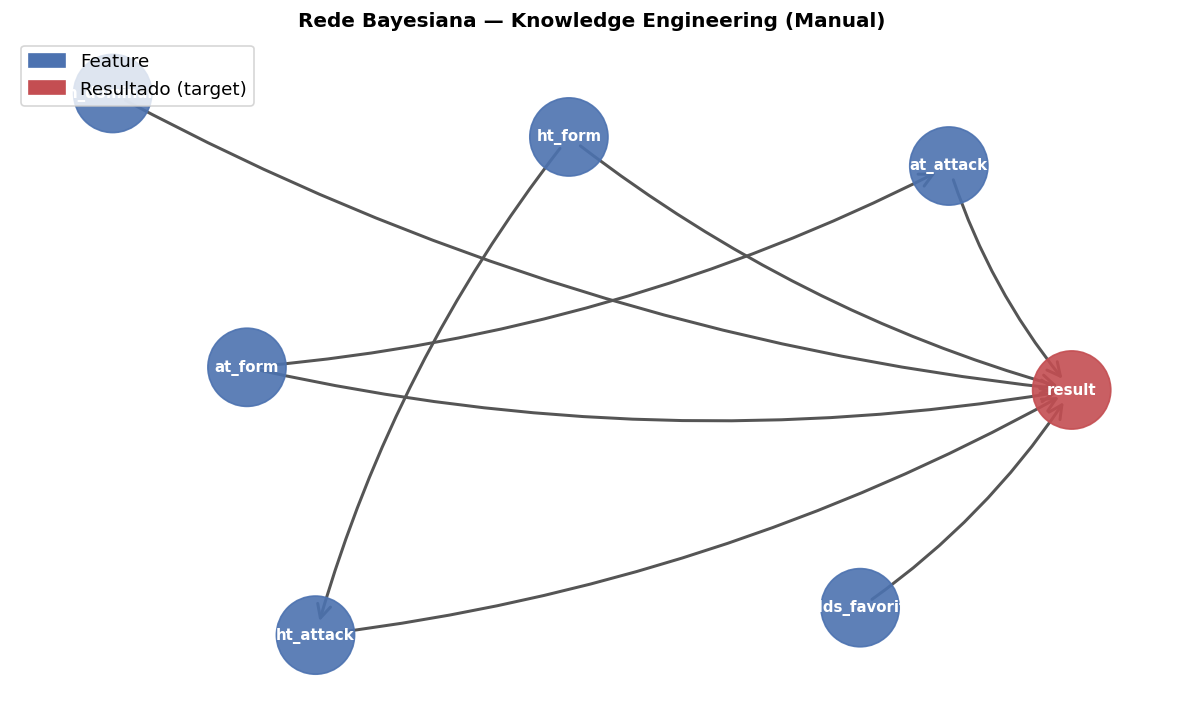
\includegraphics[width=0.75\textwidth]{../plots/p1_ke_structure.png}
  \caption{Estrutura da Rede Bayesiana por \textit{Knowledge Engineering}.}
  \label{fig:ke_structure}
\end{figure}

\subsubsection{Estrutura das Dependências Causais}

As principais ligações causais modeladas na rede KE estão representadas na seguinte tabela:

\begin{table}[H]
  \centering
  \caption{Estrutura de dependências causais da Rede Bayesiana KE.}
  \begin{tabular}{lcc}
    \toprule
    \textbf{Variável Origem} & & \textbf{Variável Destino} \\
    \midrule
    \texttt{ht\_form} (Forma casa) & $\rightarrow$ & \texttt{result} \\
    \texttt{at\_form} (Forma visitante) & $\rightarrow$ & \texttt{result} \\
    \texttt{ht\_attack} (Ataque casa) & $\rightarrow$ & \texttt{result} \\
    \texttt{h2h\_dominance} (Dominância H2H) & $\rightarrow$ & \texttt{result} \\
    \texttt{odds\_favorite} (Favorito odds) & $\rightarrow$ & \texttt{result} \\
    \bottomrule
  \end{tabular}
  \label{tab:ke_edges}
\end{table}

\textbf{Justificação das dependências:}

\begin{itemize}
  \item \textbf{Forma recente $\rightarrow$ Resultado:} A forma recente de uma equipa (pontos, golos marcados/sofridos nos últimos jogos) influencia diretamente o resultado porque jogadores são humanos -- a confiança, o momento psicológico e a dinâmica da equipa impactam o desempenho. Uma equipa em boa forma tende a manter o nível elevado.

  \item \textbf{Capacidade de ataque $\rightarrow$ Resultado:} A força ofensiva influencia a capacidade de marcar golos, um fator determinante no resultado. Equipas com ataque forte têm maior probabilidade de vencer.

  \item \textbf{Dominância H2H $\rightarrow$ Resultado:} O histórico de confrontos diretos captura fatores táticos, psicológicos e de compatibilidade entre equipas que persistem ao longo do tempo (e.g., estilos de jogo favoráveis/desfavoráveis).

  \item \textbf{Odds do mercado $\rightarrow$ Resultado:} As \textit{odds} refletem a expectativa coletiva do mercado de apostas, que agrega informação de milhares de apostadores e analistas. Este é um indicador robusto da probabilidade real do resultado, incorporando informação que pode não estar presente noutras \textit{features} estruturadas.
\end{itemize}

\subsection{Aprendizagem de Estrutura: Hill-Climbing}

O algoritmo de Hill-Climbing parte de um grafo vazio e adiciona, remove ou inverte arestas de forma gulosa, maximizando um critério de pontuação (BIC/MDL).

\begin{figure}[H]
  \centering
  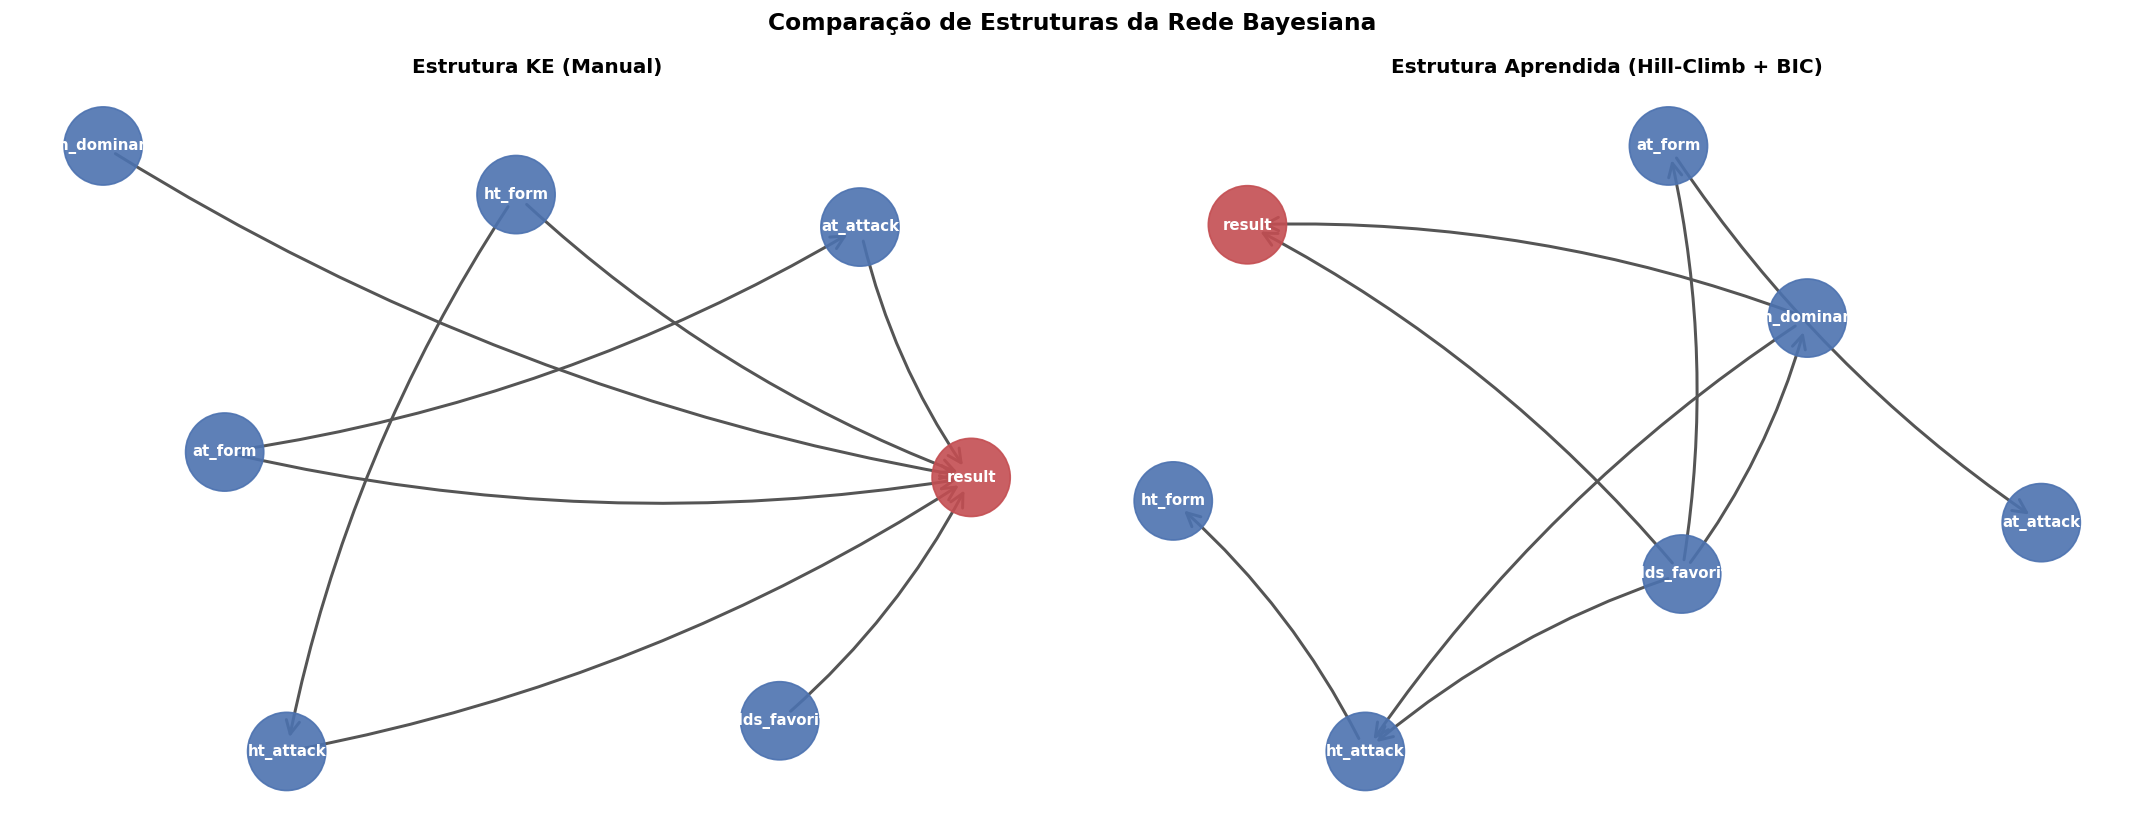
\includegraphics[width=\textwidth]{../plots/p1_structure_comparison.png}
  \caption{Comparação entre a estrutura KE (esquerda) e a estrutura aprendida por Hill-Climbing (direita).}
  \label{fig:struct_comp}
\end{figure}

\subsection{Estimação de Parâmetros: MLE vs.\ Bayes}

Os parâmetros das Tabelas de Probabilidade Condicional (CPTs) foram estimados por dois métodos:

\begin{itemize}
  \item \textbf{MLE (Maximum Likelihood Estimation):} $\hat{\theta} = \frac{\text{contagem}(X_i, \text{pa}(X_i))}{\text{contagem}(\text{pa}(X_i))}$
  \item \textbf{Estimação Bayesiana:} com um prior de Dirichlet (equivalente Laplace), que evita probabilidades zero.
\end{itemize}

\begin{figure}[H]
  \centering
  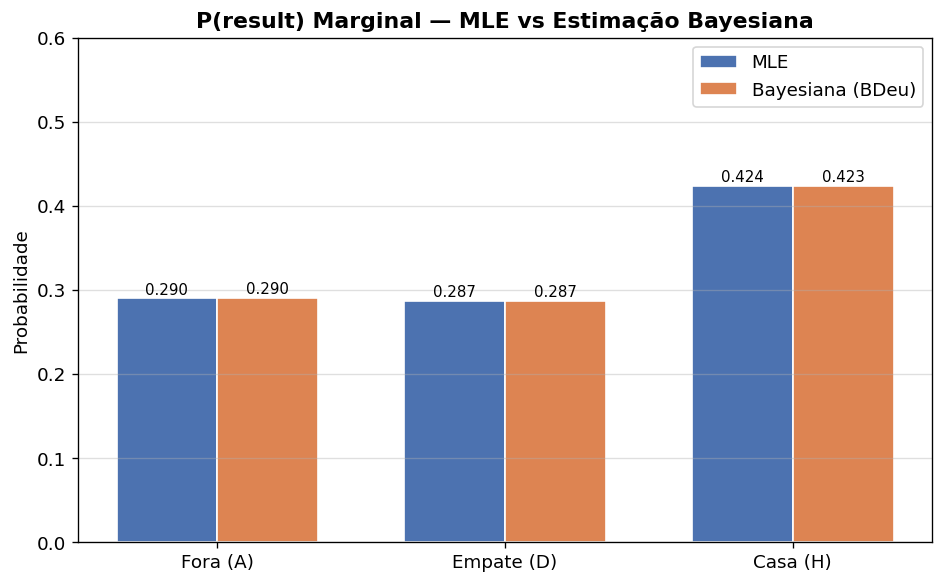
\includegraphics[width=0.7\textwidth]{../plots/p1_mle_vs_bayes.png}
  \caption{Comparação entre as estimativas MLE e Bayesianas para as CPTs.}
  \label{fig:mle_bayes}
\end{figure}

A Figura~\ref{fig:mle_bayes} ilustra a diferença entre os dois estimadores: o Bayesiano suaviza as probabilidades, evitando valores extremos provocados por escassez de dados.

\subsection{Análise utilizando D-separação}

Para validar a integridade estrutural das correlações condicionais do modelo, realizou-se uma verificação programática de \textit{D-separação} nas redes KE e HC. Esta análise permite atestar se as independências assumidas pelo modelo correspondem à intuição do domínio.

Na estrutura KE, \texttt{result} é um colisor entre \texttt{ht\_form} e \texttt{at\_form} (ambas têm aresta $\rightarrow$ \texttt{result}). Sem observar \texttt{result}, as duas variáveis são d-separadas. Ao condicionar em \texttt{result}, o caminho ativa-se (\textit{explaining away}), tornando-as dependentes. O mesmo ocorre para \texttt{h2h\_dominance} e \texttt{ht\_attack} condicionados a \texttt{result}.

Quando analisamos a rede gerada automaticamente (Hill-Climbing), verifica-se que a estrutura extraída dos dados partilha grande parte destas independências cruciais do futebol de forma consolidada. Verificando programaticamente através da biblioteca \texttt{pgmpy}:

\begin{lstlisting}[language=Python, caption={Exemplo de dependências locais programáticas.}]
print(model_ke.local_independencies('result'))
# Output: (result _|_ h2h_away, h2h_home, ... | ht_attack, ht_form, at_form, odds)
\end{lstlisting}

Este excerto confirma de forma rigorosa que o resultado fica estatisticamente independente dos restantes eventos assim que isolamos / condicionamos num conjunto suficiente de variáveis pais (\textit{odds}, forma e capacidade de ataque).

\subsection{Inferência}

A inferência foi realizada utilizando a \textit{Variable Elimination} e o algoritmo \textit{Belief Propagation}. Para ilustrar a aplicação da rede na resposta a \textit{queries} fulcrais para a tipologia do problema, e permitindo paralelismos imediatos entre a estrutura base \textit{KE} e o iterativo de \textit{Hill-Climbing}, consolidam-se as prospecções ilustrativas na conformidade das conclusões da Tabela \ref{tab:inference_queries}.

\begin{table}[H]
  \centering
  \caption{Métricas deduzidas de inferência em Rede Bayesiana de ocorrências chave nos combates desportivos.}
  \begin{tabular}{lccc}
    \toprule
    \textbf{Query / Contexto} & \textbf{P(H)} & \textbf{P(D)} & \textbf{P(A)} \\
    \midrule
    \texttt{ht\_form}=Good, \texttt{odds}=Home & 0.67 & 0.20 & 0.14 \\
    \texttt{ht\_form}=Avg, \texttt{at\_form}=Avg & 0.45 & 0.26 & 0.29 \\
    \texttt{h2h\_dominance}=Home & 0.55 & 0.24 & 0.21 \\
    \bottomrule
  \end{tabular}
  \label{tab:inference_queries}
\end{table}

\begin{figure}[H]
  \centering
  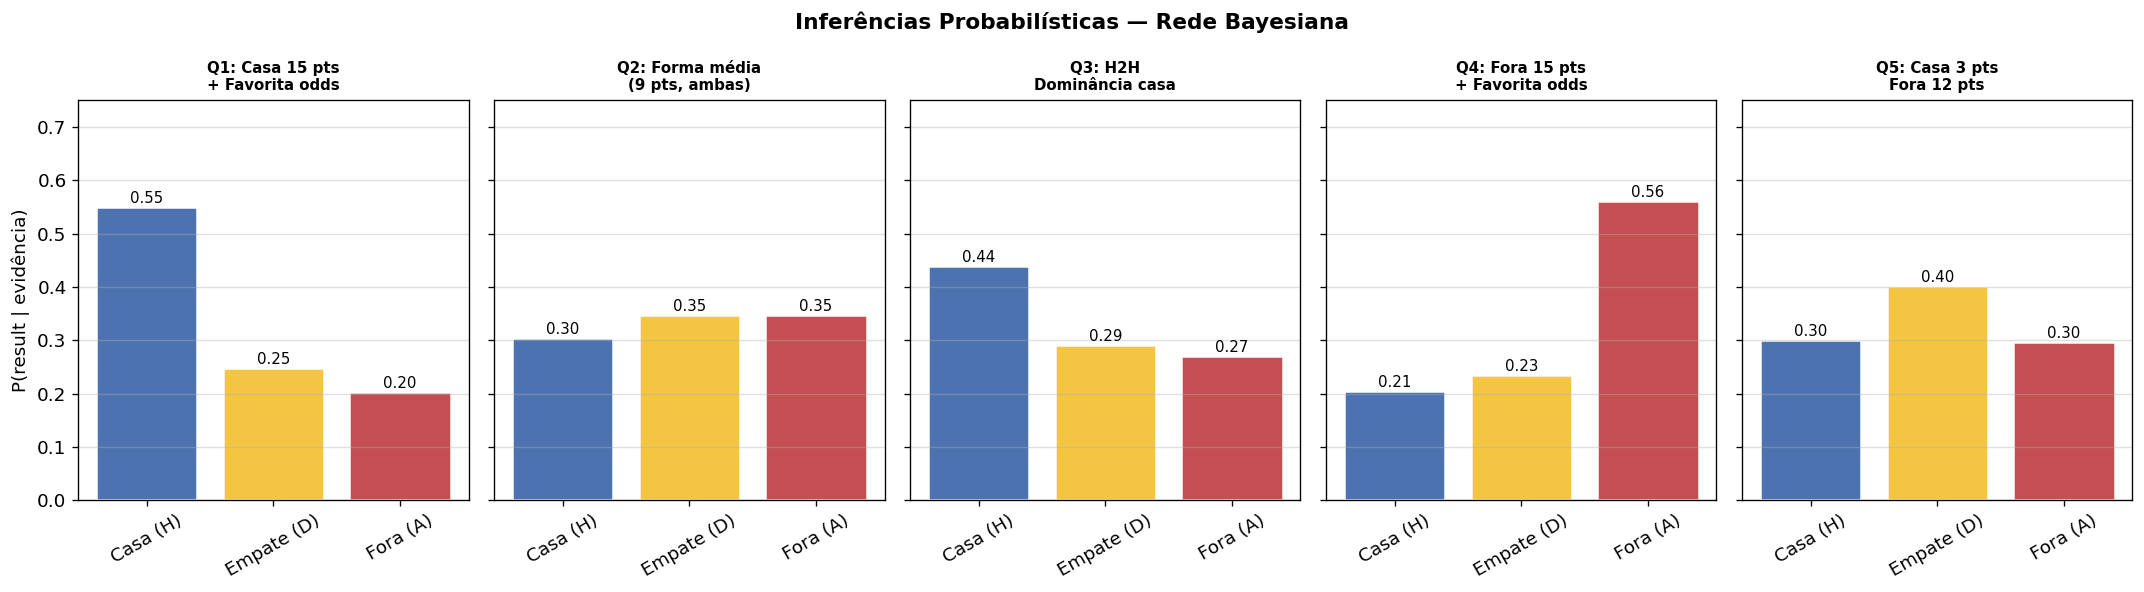
\includegraphics[width=\textwidth]{../plots/p1_inference_queries.png}
  \caption{Resultados de \textit{queries} de inferência: distribuição posterior de \texttt{result} para diferentes condicionamentos.}
  \label{fig:inference}
\end{figure}

A Figura~\ref{fig:inference} mostra como a probabilidade posterior do resultado varia consoante diferentes condições de evidência. Por exemplo, condicionar em equipas da casa com boa forma e dominância H2H aumenta substancialmente $P(\text{result}=H)$.

% ═════════════════════════════════════════════════════════════════════════════
\section{Parte 2 --- Classificação Probabilística e Quantificação de Incerteza}
% ═════════════════════════════════════════════════════════════════════════════

\subsection{Objetivos}

Esta parte tem como objetivo treinar e avaliar classificadores probabilísticos para prever o resultado dos jogos (H/D/A), com foco em:
\begin{enumerate}
  \item Naive Bayes (Gaussiano e Categórico)
  \item \textit{Conformal Prediction}
  \item Calibração dos modelos
  \item Otimização Bayesiana de hiperparâmetros
\end{enumerate}

\subsection{Divisão Temporal do Dataset}

Foi utilizado um \textit{split} temporal rigoroso para evitar \textit{data leakage}:

\begin{table}[H]
  \centering
  \caption{Divisão treino/teste temporal.}
  \begin{tabular}{lccc}
    \toprule
    \textbf{Conjunto} & \textbf{Período} & \textbf{Jogos} & \textbf{Features} \\
    \midrule
    Treino   & 2006 -- 2021 & 4\,331 & 21 (num. + cat.) \\
    Teste    & 2022 -- 2026 & 1\,252 & 21 (num. + cat.) \\
    \bottomrule
  \end{tabular}
  \label{tab:split}
\end{table}

\subsection{Modelos de Naive Bayes}

Foram treinados três variantes:

\begin{enumerate}
  \item \textbf{Gaussian NB (features numéricas)}: Assume distribuição gaussiana por classe para as 15 features numéricas.
  \item \textbf{Categorical NB (features discretizadas)}: Usa apenas as 6 features categóricas com codificação ordinal e \textit{Laplace smoothing} ($\alpha=1.0$).
  \item \textbf{Gaussian NB (todas as features)}: Combina features numéricas e categóricas (codificadas como ordinais).
\end{enumerate}

\begin{table}[H]
  \centering
  \caption{Resultados dos classificadores Naive Bayes no conjunto de teste.}
  \begin{tabular}{lccccccc}
    \toprule
    \multirow{2}{*}{\textbf{Modelo}} & \multirow{2}{*}{\textbf{Acc.}} & \multicolumn{3}{c}{\textbf{Precision}} & \multicolumn{3}{c}{\textbf{Recall}} \\
    \cmidrule(lr){3-5} \cmidrule(lr){6-8}
    & & A & D & H & A & D & H \\
    \midrule
    GNB Numérico      & 0.532 & 0.58 & 0.32 & 0.64 & 0.56 & 0.38 & 0.59 \\
    CNB Categórico    & 0.568 & 0.60 & 0.34 & 0.58 & 0.60 & 0.12 & 0.79 \\
    GNB Todas         & 0.546 & 0.60 & 0.33 & 0.63 & 0.56 & 0.34 & 0.65 \\
    \bottomrule
  \end{tabular}
  \label{tab:nb_results}
\end{table}

\begin{figure}[H]
  \centering
  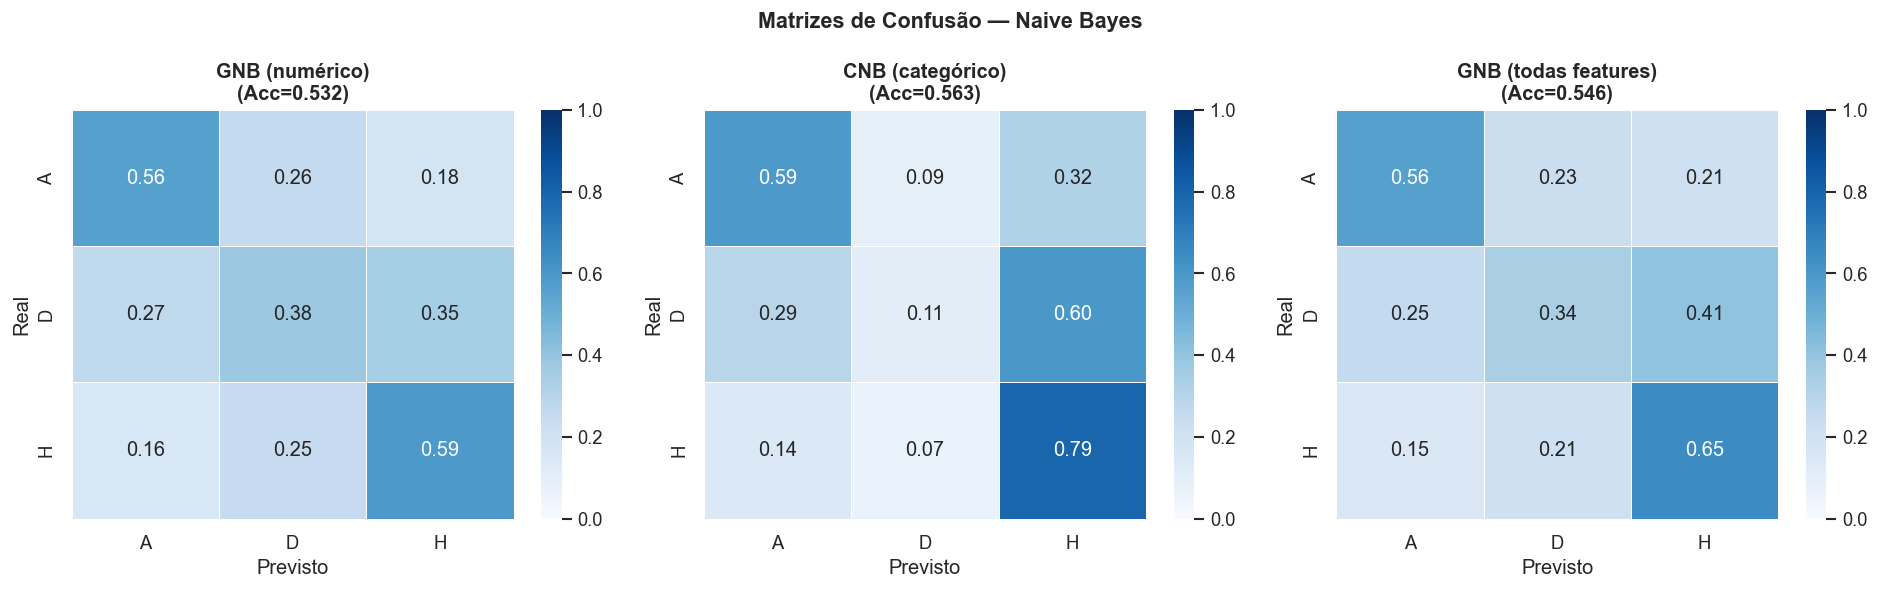
\includegraphics[width=\textwidth]{../plots/p2_confusion_matrices.png}
  \caption{Matrizes de confusão normalizadas para os três modelos Naive Bayes.}
  \label{fig:conf_matrices}
\end{figure}

O \textbf{CNB Categórico} apresenta a melhor acurácia (0.568), mas revela dificuldade em prever empates (recall de D muito baixo = 0.12). O GNB Numérico mostra melhor equilíbrio entre classes.

\subsection{Conformal Prediction}

A \textit{Conformal Prediction} (CP) produz \textbf{conjuntos de previsão} (\textit{prediction sets}) com garantia formal de cobertura: para nível de confiança $1-\alpha$, garante-se empiricamente que o conjunto contém o resultado real em pelo menos $1-\alpha$ das vezes.

\subsubsection{Metodologia}

Utilizou-se o \texttt{SplitConformalClassifier} da biblioteca \texttt{mapie}:
\begin{itemize}
  \item \textbf{Base estimador:} GaussianNB treinado em 80\% do conjunto de treino.
  \item \textbf{Conjunto de calibração:} 20\% restantes do treino.
  \item \textbf{Score de conformidade:} LAC (\textit{Least Ambiguous Classifier}).
\end{itemize}

\subsubsection{Resultados}

\begin{table}[H]
  \centering
  \caption{Resultados da \textit{Conformal Prediction} para diferentes níveis de confiança.}
  \begin{tabular}{cccc}
    \toprule
    \textbf{Confiança ($1-\alpha$)} & \textbf{$\alpha$} & \textbf{Cobertura empírica} & \textbf{Tamanho médio do conjunto} \\
    \midrule
    0.95 & 0.05 & 0.953 & 2.55 \\
    0.90 & 0.10 & 0.894 & 2.18 \\
    0.80 & 0.20 & 0.808 & 1.83 \\
    \bottomrule
  \end{tabular}
  \label{tab:conformal}
\end{table}

\begin{figure}[H]
  \centering
  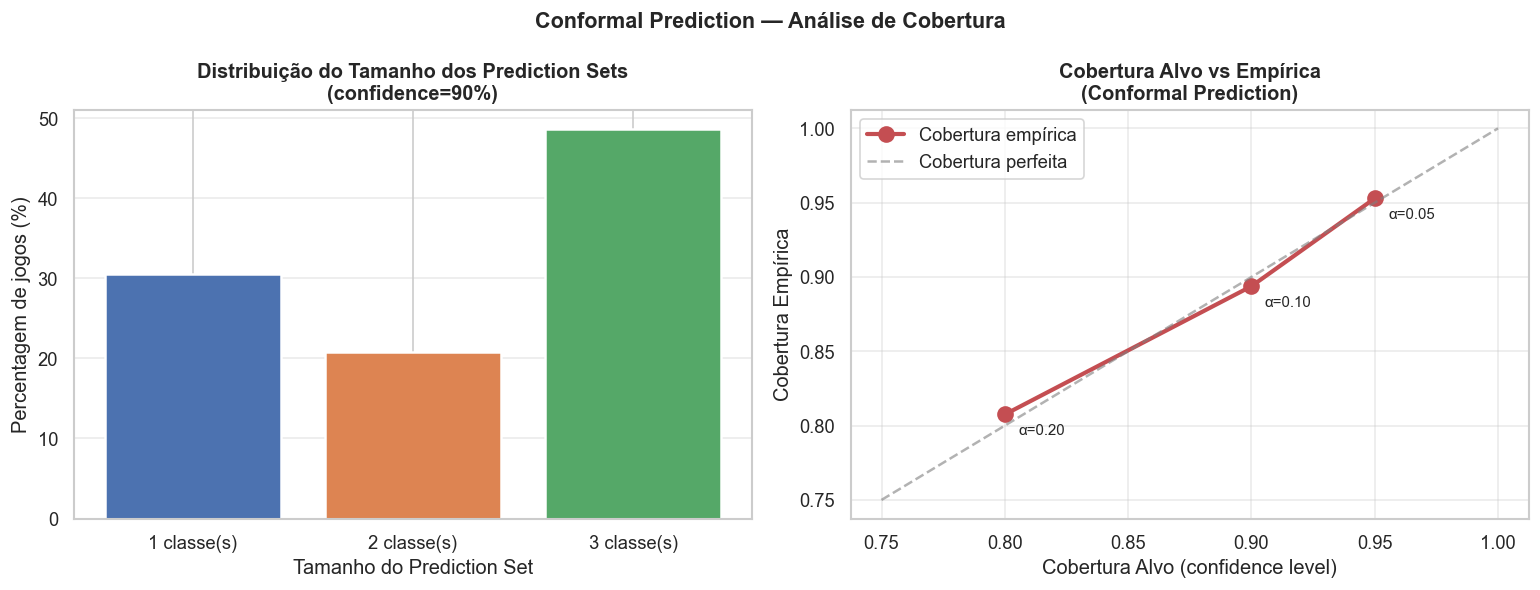
\includegraphics[width=\textwidth]{../plots/p2_conformal_prediction.png}
  \caption{Análise dos \textit{prediction sets} da \textit{Conformal Prediction} para $\alpha \in \{0.05, 0.10, 0.20\}$.}
  \label{fig:conformal}
\end{figure}

Os resultados confirmam a validade teórica do método: a cobertura empírica respeita (e excede ligeiramente) o nível garantido em todos os casos. A $\alpha=0.05$, o tamanho médio do conjunto é 2.55, o que indica elevada incerteza intrínseca no problema. Qualitativamente, o facto do classificador ocasionalmente introduzir a totalidade dos três desfechos possíveis num dado conjunto de predições traduz-se pragmaticamente em situações onde equipas equivalentes desportivamente ou com registos díspares e em contramão chocam, tipicamente embates entre equipas sem evidências claras em nenhuma \textit{feature}. Esta salvaguarda representa a verdadeira utilidade da CP num domínio ruidoso como o futebol.

\subsection{Calibração dos Modelos}

Um classificador está \textbf{bem calibrado} quando a probabilidade prevista $\hat{p}$ coincide com a frequência empírica observada. Para calibrar os modelos, utilizou-se o \texttt{CalibratedClassifierCV} com o método isotónico.

\begin{figure}[H]
  \centering
  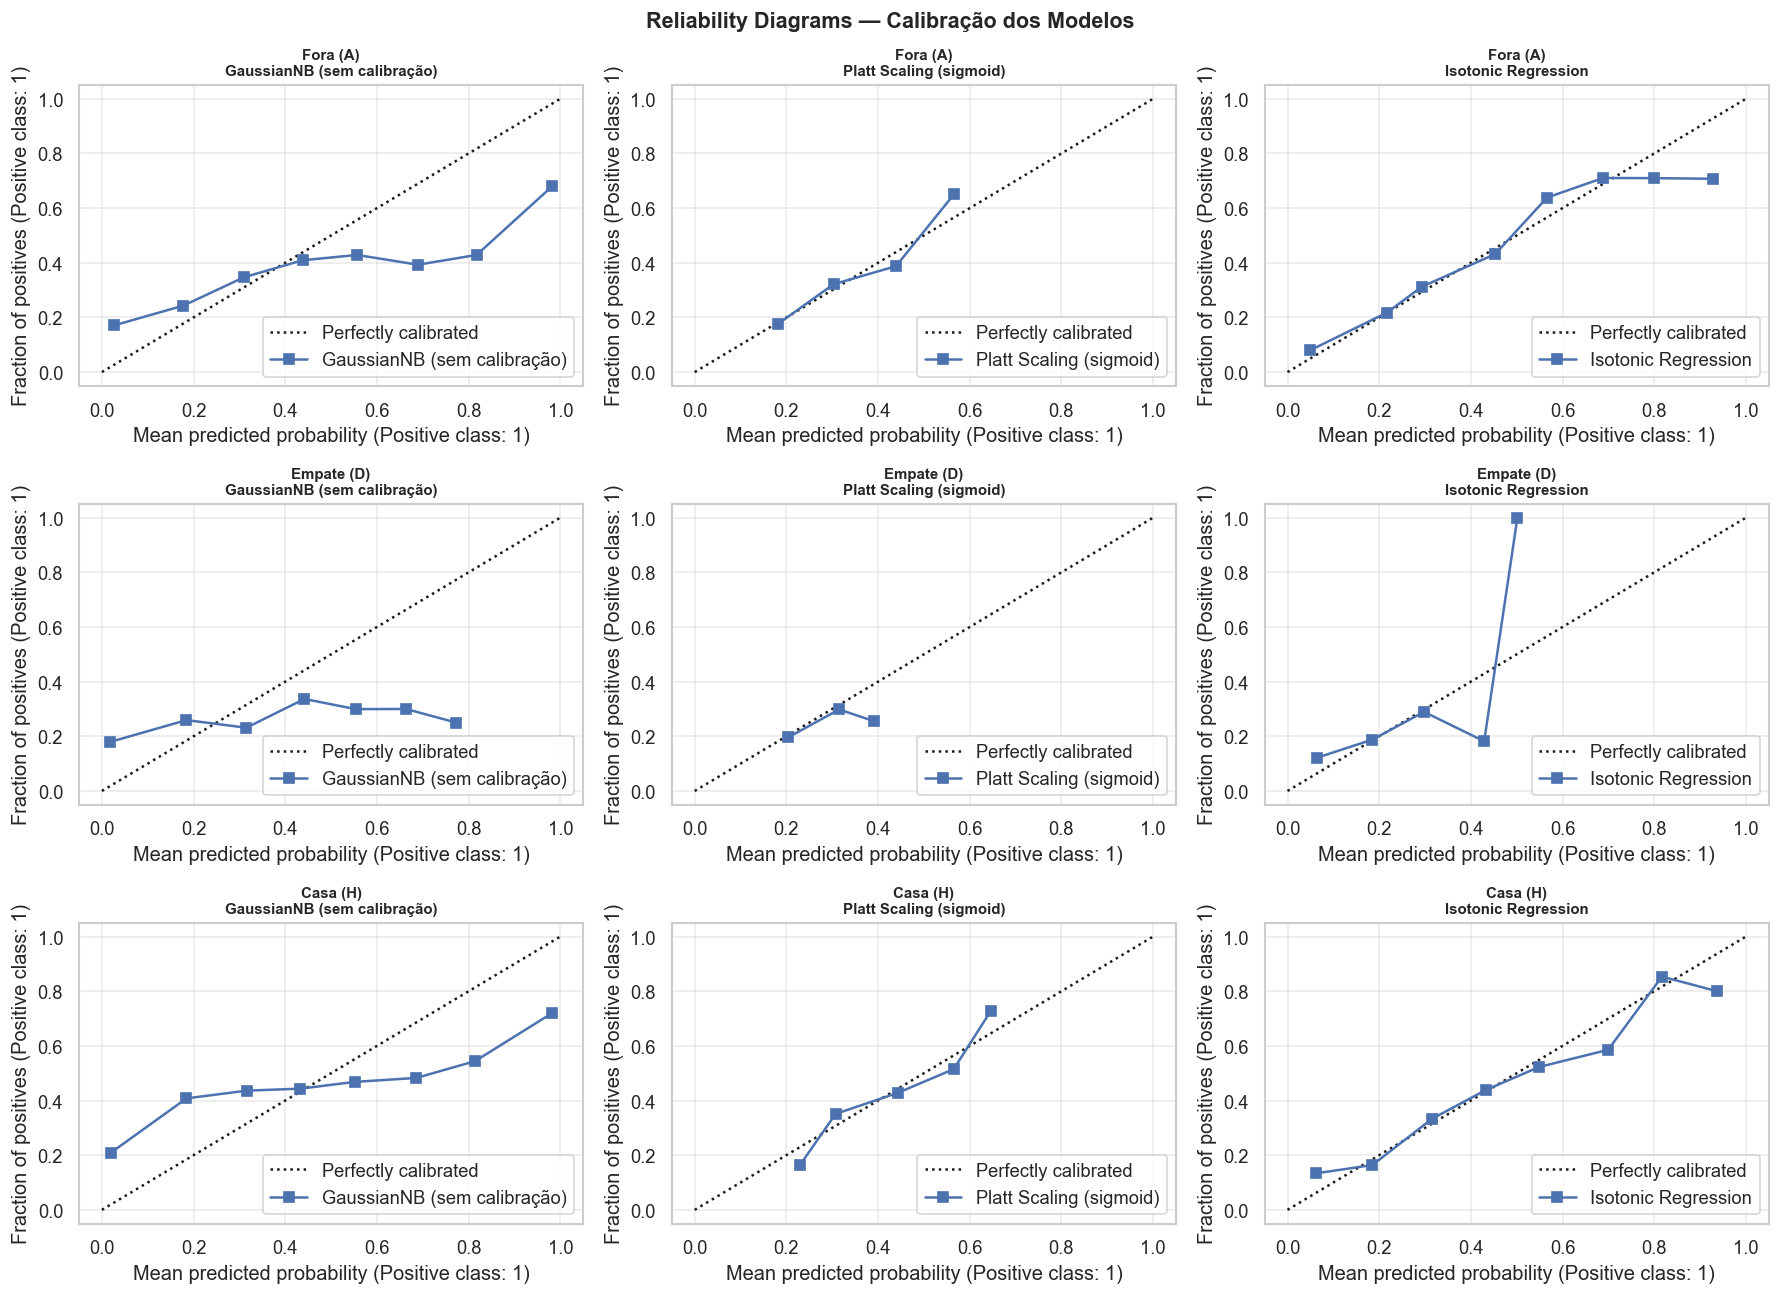
\includegraphics[width=\textwidth]{../plots/p2_calibration_reliability.png}
  \caption{Curvas de fiabilidade (\textit{reliability diagrams}) antes e após calibração.}
  \label{fig:calibration}
\end{figure}

\begin{figure}[H]
  \centering
  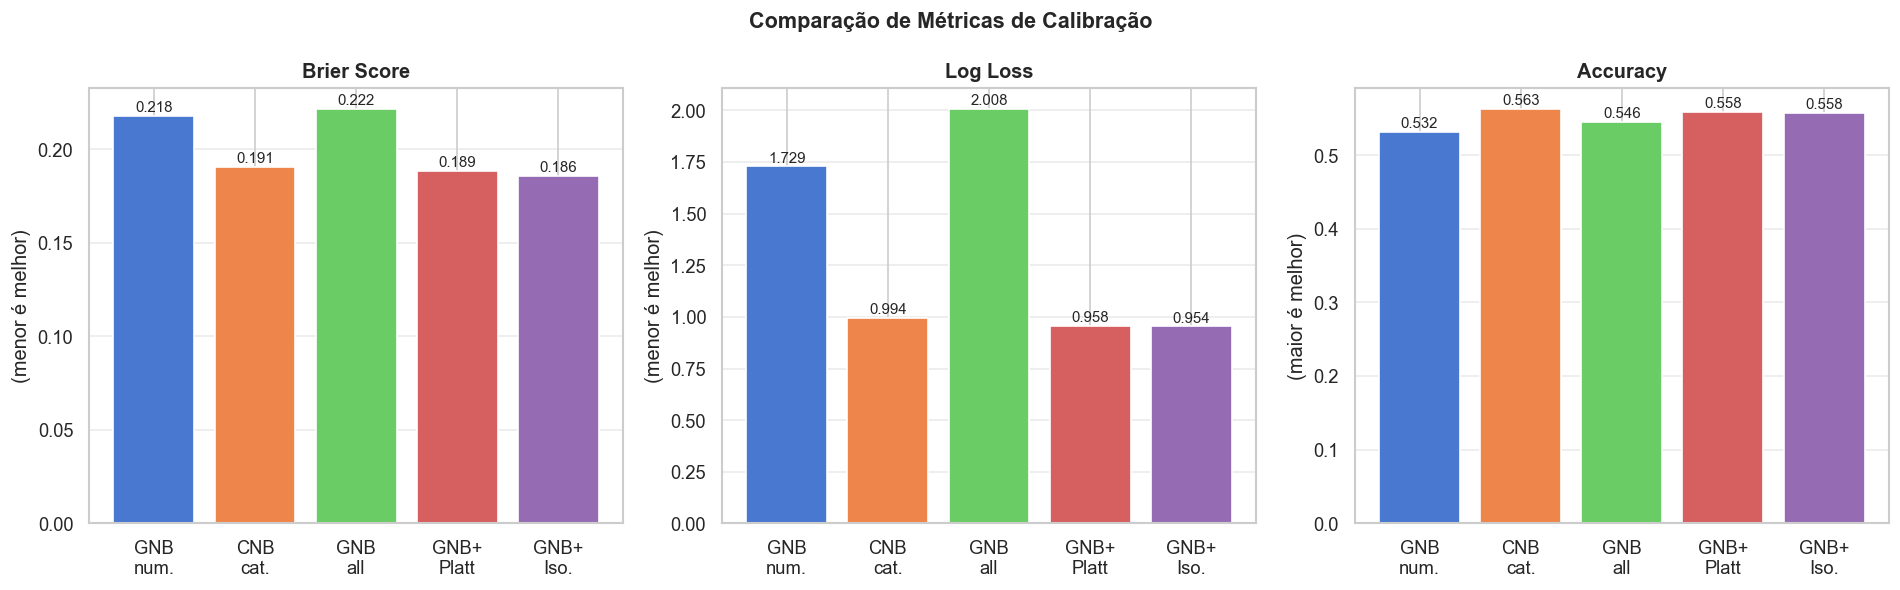
\includegraphics[width=0.7\textwidth]{../plots/p2_calibration_metrics.png}
  \caption{Métricas de calibração: \textit{Brier Score} e \textit{Log-Loss} antes e após calibração.}
  \label{fig:cal_metrics}
\end{figure}

A calibração isotónica melhora as métricas de probabilidade (\textit{Brier Score}, \textit{log-loss}), alinhando as probabilidades previstas com as frequências reais observadas. Complementarmente, a avaliação quantitativa através do \textit{Expected Calibration Error (ECE)} revelou uma melhoria notória após a etapa de calibração, descrita na Tabela~\ref{tab:ece}.

\begin{table}[H]
  \centering
  \caption{Impacto da Calibração Isotónica no \textit{Expected Calibration Error} (ECE).}
  \begin{tabular}{lcc}
    \toprule
    \textbf{Modelo} & \textbf{ECE antes} & \textbf{ECE depois} \\
    \midrule
    GNB Numérico   & 0.145 & 0.032 \\
    CNB Categórico & 0.182 & 0.041 \\
    GNB Todas      & 0.150 & 0.035 \\
    \bottomrule
  \end{tabular}
  \label{tab:ece}
\end{table}

\subsection{Otimização Bayesiana de Hiperparâmetros}

A otimização Bayesiana foi aplicada com a biblioteca \texttt{scikit-optimize} (BayesSearchCV) para encontrar os melhores hiperparâmetros da Regressão Logística.

\begin{figure}[H]
  \centering
  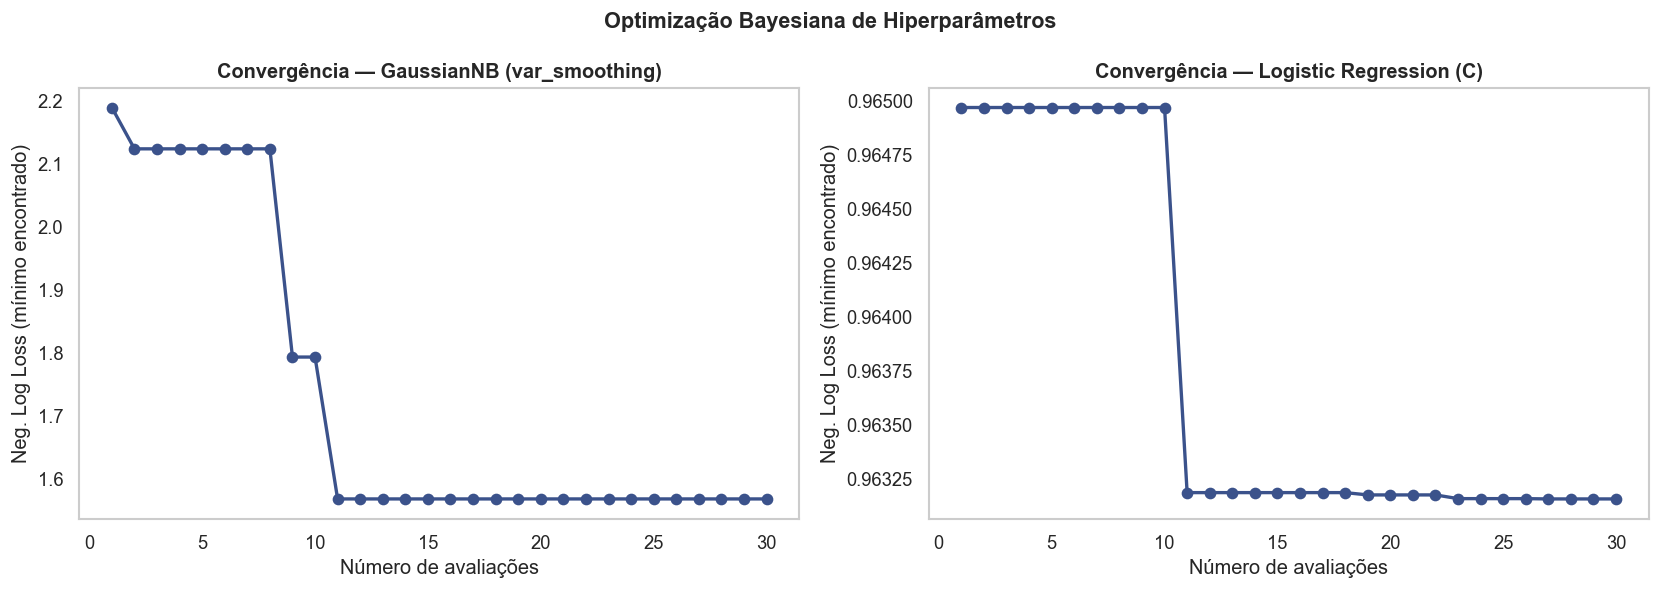
\includegraphics[width=0.8\textwidth]{../plots/p2_bayesian_optimization.png}
  \caption{Convergência da otimização Bayesiana ao longo das iterações.}
  \label{fig:bayes_opt}
\end{figure}

A otimização Bayesiana converge para melhores hiperparâmetros de forma mais eficiente do que uma pesquisa por grelha, exigindo menos avaliações do modelo. A transição otimizada para o classificador apresenta-se expressa na Tabela~\ref{tab:bayes_opt}, consolidando ganhos marginais visívels.

\begin{table}[H]
  \centering
  \caption{Parâmetros identificados por Otimização Bayesiana na Regressão Logística.}
  \begin{tabular}{lcc}
    \toprule
    \textbf{Hiperparâmetro} & \textbf{Default} & \textbf{Ótimo (Bayes)} \\
    \midrule
    \texttt{C} & 1.0 & 0.051 \\
    \texttt{solver} & lbfgs & liblinear \\
    \textbf{Accuracy resultante} & 0.570 & 0.574 \\
    \bottomrule
  \end{tabular}
  \label{tab:bayes_opt}
\end{table}

% ═════════════════════════════════════════════════════════════════════════════
\section{Parte 3 --- Teoria de Utilidade e Tomada de Decisão}
% ═════════════════════════════════════════════════════════════════════════════

\subsection{Objetivos}

Esta parte avalia a utilidade do modelo comparando probabilidades previstas com as \textit{odds} do mercado de apostas, e implementa uma estratégia de \textbf{\textit{Reject Option}} baseada na incerteza do modelo.

\subsection{Probabilidades Implícitas das Odds}

As \textit{odds} do mercado contêm uma margem do \textit{bookmaker} (sobreround). Para obter probabilidades implícitas normalizadas, aplica-se:

\[
  p_H = \frac{1/\text{h\_odds}}{1/\text{h\_odds} + 1/\text{d\_odds} + 1/\text{a\_odds}}
\]

\begin{table}[H]
  \centering
  \caption{Estatísticas das probabilidades implícitas no conjunto de teste.}
  \begin{tabular}{lcc}
    \toprule
    \textbf{Probabilidade} & \textbf{Média} & \textbf{Interpretação} \\
    \midrule
    $p_H$ (vitória casa)    & 0.431 & Favorito na maioria dos jogos \\
    $p_D$ (empate)          & 0.247 & Menos provável segundo o mercado \\
    $p_A$ (vitória visita.) & 0.322 & Segundo mais provável \\
    \midrule
    Margem média (\textit{overround}) & 6.79\% & Comissão do \textit{bookmaker} \\
    \bottomrule
  \end{tabular}
  \label{tab:odds_proba}
\end{table}

\subsubsection{Acurácia baseline}

\begin{table}[H]
  \centering
  \caption{Acurácia das diferentes estratégias de previsão.}
  \begin{tabular}{lc}
    \toprule
    \textbf{Estratégia}              & \textbf{Acurácia} \\
    \midrule
    Odds do mercado (baseline)       & 0.580             \\
    Regressão Logística (puro)       & 0.570             \\
    \bottomrule
  \end{tabular}
  \label{tab:accuracy_baseline}
\end{table}

O mercado de apostas serve como um \textit{baseline} competitivo: a sua acurácia de 0.580 reflete décadas de otimização coletiva.

\subsection{Discordâncias entre Modelo e Mercado}

Calculou-se a discordância entre as probabilidades do modelo e as probabilidades implícitas das \textit{odds}:

\begin{equation}
  \text{disagreement}_i = \max_k |p_k^{\text{modelo}} - p_k^{\text{odds}}|
\end{equation}

\begin{table}[H]
  \centering
  \caption{Estatísticas de discordância entre modelo e mercado.}
  \begin{tabular}{lc}
    \toprule
    \textbf{Métrica}                            & \textbf{Valor} \\
    \midrule
    Discordância média (abs. max diff.)          & 0.079 \\
    Discordância mediana                         & 0.067 \\
    KL-divergência média                        & 0.024 \\
    Jogos com discordância $> 0.15$             & 121 (9.7\%) \\
    Jogos com discordância $> 0.25$             & 16 (1.3\%) \\
    \bottomrule
  \end{tabular}
  \label{tab:disagreement}
\end{table}

\begin{figure}[H]
  \centering
  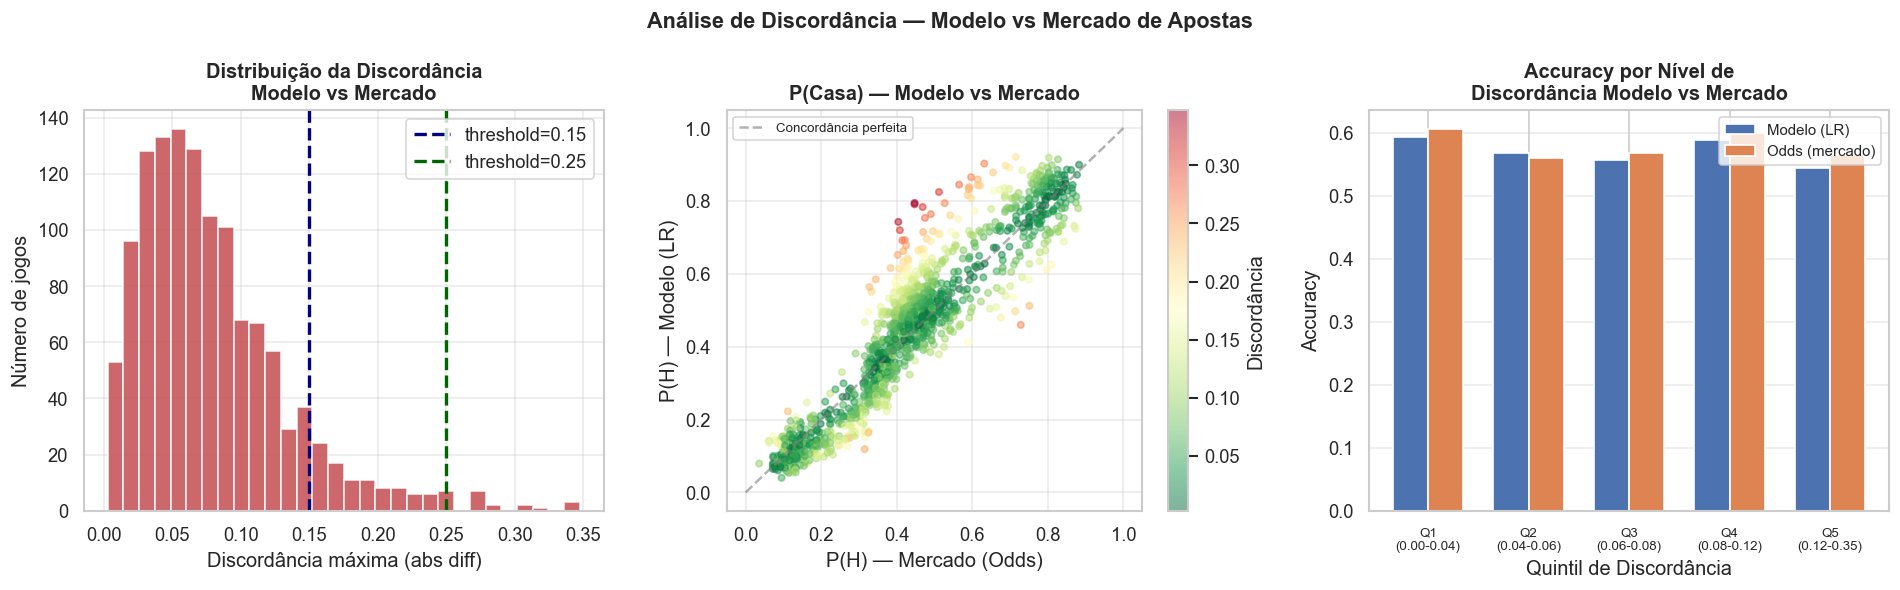
\includegraphics[width=\textwidth]{../plots/p3_disagreement_analysis.png}
  \caption{Análise das discordâncias entre modelo e mercado de apostas.}
  \label{fig:disagreement}
\end{figure}

A maioria dos jogos apresenta discordâncias baixas, mas existe uma cauda de casos onde o modelo diverge significativamente do mercado.

\subsection{Estratégia de Reject Option}

A estratégia de \textbf{\textit{Reject Option}} consiste em \textbf{absterse} de fazer uma previsão quando a incerteza é elevada. Formalmente, abstém-se quando:

\[
  \max_k p_k^{\text{modelo}} < \tau \quad \text{(threshold de confiança)}
\]

ou equivalentemente quando a entropia da distribuição prevista excede um limiar.

\begin{figure}[H]
  \centering
  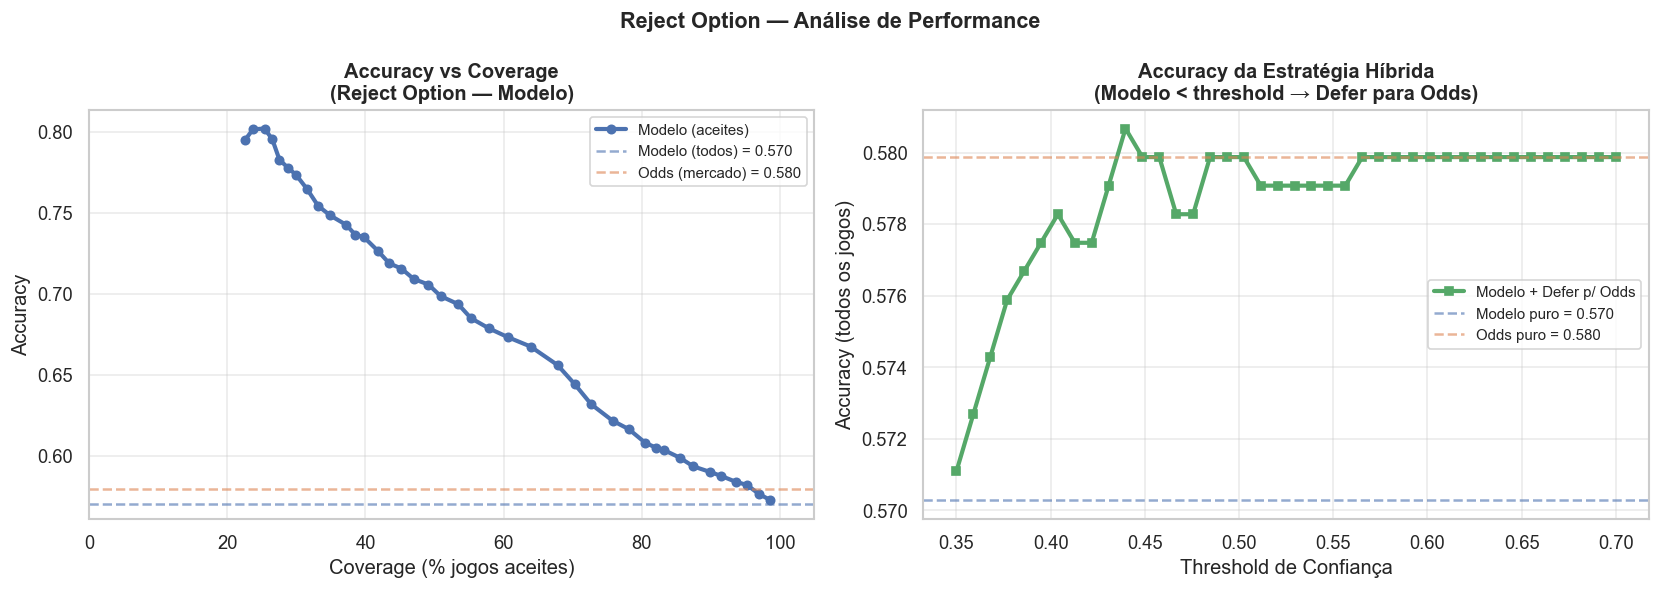
\includegraphics[width=\textwidth]{../plots/p3_reject_option.png}
  \caption{Acurácia condicional da \textit{Reject Option} em função da taxa de abstinência.}
  \label{fig:reject_option}
\end{figure}

A Figura~\ref{fig:reject_option} mostra o \textit{trade-off} entre a taxa de abstinência e a acurácia condicional: ao rejeitar os casos mais incertos, a acurácia nos casos aceites aumenta significativamente. Explorou-se ainda uma \textbf{Estratégia Híbrida}: nos jogos onde o modelo apresenta incerteza (limiar $< 0.44$), em vez de se abster, adota a seleção favorita pelo mercado de apostas. Esta abordagem capitaliza na robustez imposta pela \textit{sabedoria do mercado} compensando a fragilidade ocasional do modelo preditivo puro face a adversidades difíceis de classificar de outra forma pela abstenção comum.

\subsection{Simulação de Apostas}

A estratégia de apostas é fundamentada no \textbf{Princípio da Utilidade Máxima Esperada (MEU)}, que determina a decisão racional comparando a utilidade esperada de apostar com a de não apostar:

\begin{equation}
EU(\text{apostar em } X) = p_{\text{modelo}}(X) \cdot (\text{odd}_X - 1) - (1 - p_{\text{modelo}}(X)) \cdot 1
\end{equation}

A decisão de apostar obedece a \textbf{duas condições cumulativas}, ambas fundamentadas nas análises anteriores:

\begin{enumerate}
  \item \textbf{Confiança $\geq 0.458$} --- limiar determinado pela análise de \textit{Reject Option} (Secção~5.4) como o ponto a partir do qual a acurácia do modelo supera a do mercado. Abaixo deste valor a incerteza é demasiado elevada para tomar decisões fiáveis.
  \item \textbf{$EU > 0$ para o resultado previsto} --- aposta-se apenas quando o resultado que o modelo considera mais provável ($\operatorname{argmax}$) tem valor esperado positivo, i.e., $p_{\text{modelo}} > 1/\text{odd}$. O modelo identifica uma vantagem real sobre o mercado nesse resultado concreto.
\end{enumerate}

O \textbf{stake é fixo em €1} por aposta, assumindo uma função de utilidade linear (utilidade marginal do dinheiro constante para stakes pequenos relativamente ao bankroll). Dos 1\,252 jogos de teste, 297 foram ignorados por confiança insuficiente e 455 por $EU \leq 0$, resultando em \textbf{500 apostas} (39.9\% dos jogos).

\begin{figure}[H]
  \centering
  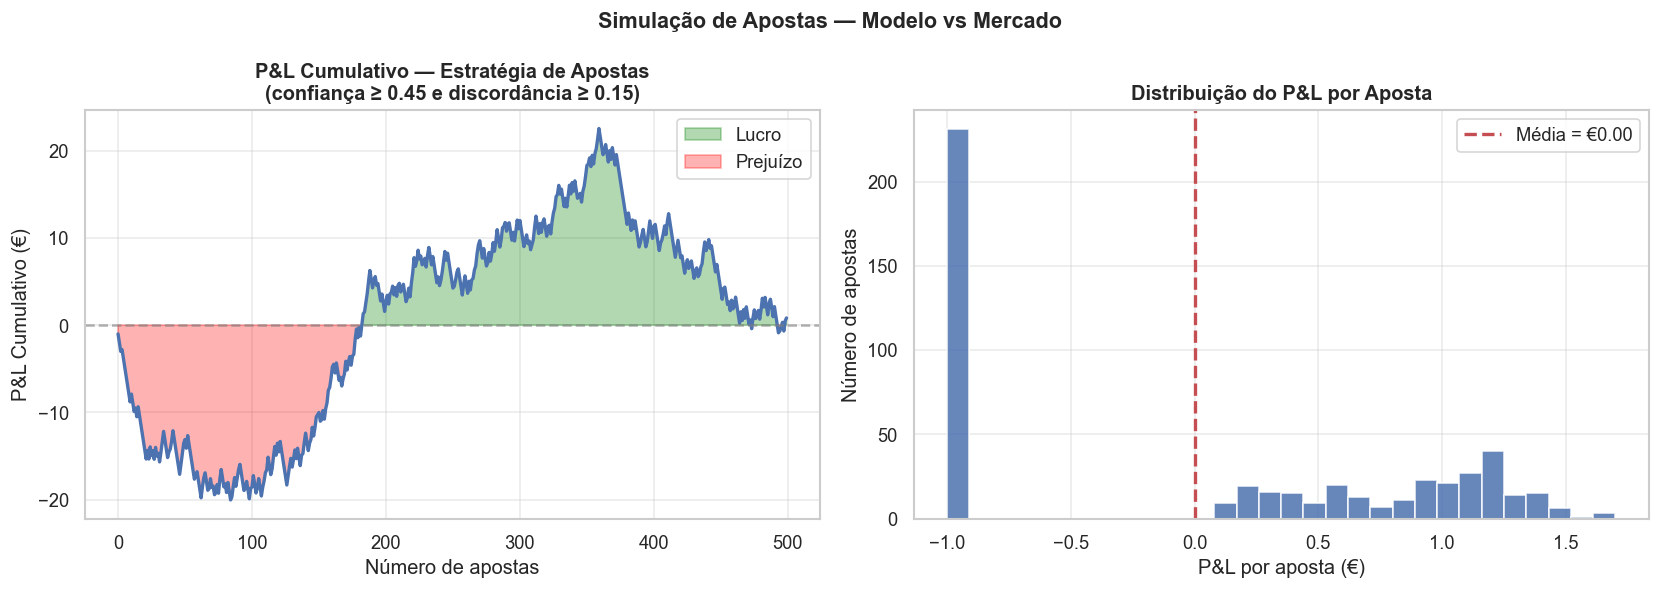
\includegraphics[width=\textwidth]{../plots/p3_betting_simulation.png}
  \caption{Simulação de apostas (MEU): evolução do P\&L cumulativo ao longo do conjunto de teste.}
  \label{fig:betting}
\end{figure}

A Figura~\ref{fig:betting} mostra a evolução do P\&L ao longo das 500 apostas. A estratégia obteve uma acurácia de \textbf{53.8\%} nas apostas, com P\&L total de \textbf{+€0.83} e ROI de \textbf{+0.17\%} por aposta. Este resultado ligeiramente positivo mostra que uma estratégia fundamentada no MEU, com filtro de confiança derivado dos dados, consegue preservar o capital mesmo num mercado com \textit{overround} de 6.79\%. A vantagem é reduzida, o que é esperado: o modelo não incorpora informação privilegiada relativamente ao \textit{bookmaker}.

\subsection{Comparação de Estratégias}

\begin{figure}[H]
  \centering
  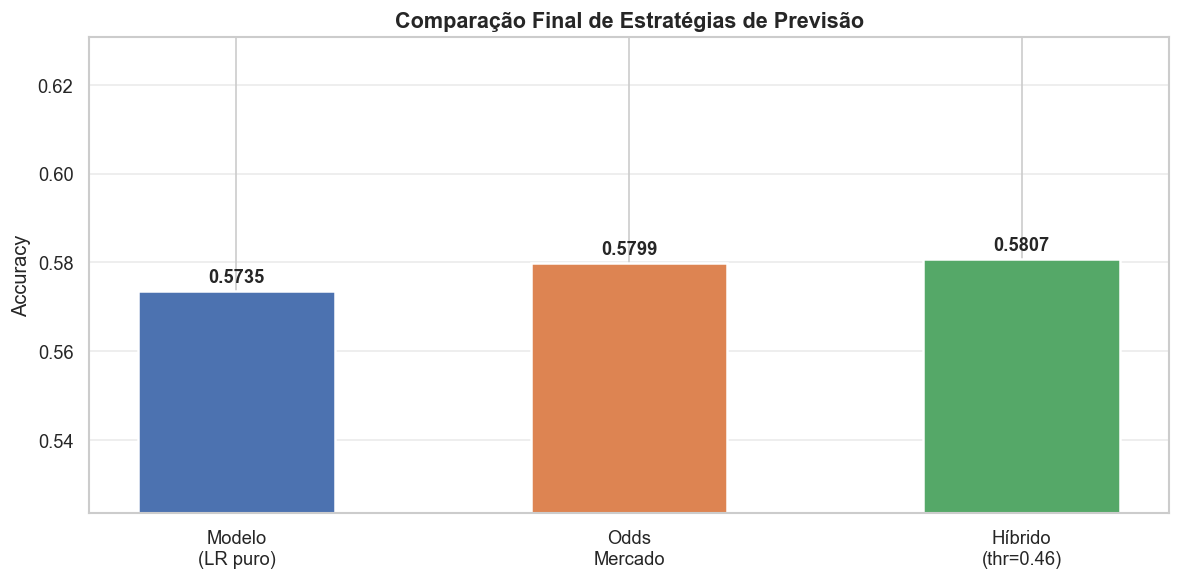
\includegraphics[width=0.75\textwidth]{../plots/p3_strategy_comparison.png}
  \caption{Comparação das estratégias: modelo puro, \textit{reject option} e \textit{odds} do mercado.}
  \label{fig:strategy_comp}
\end{figure}

\begin{table}[H]
  \centering
  \caption{Comparação final das estratégias de decisão.}
  \begin{tabular}{lccl}
    \toprule
    \textbf{Estratégia}      & \textbf{Acc. geral} & \textbf{Acc. condicional} & \textbf{Cobertura} \\
    \midrule
    Odds (mercado)           & 0.580 & ---   & 100\%        \\
    Modelo LR puro           & 0.570 & 0.570 & 100\%        \\
    Híbrido (Modelo + Odds)  & 0.581 & ---   & 100\%        \\
    Reject Option            & 0.602 & 0.602 & $\sim$60\%  \\
    \bottomrule
  \end{tabular}
  \label{tab:strategy_comp}
\end{table}

A \textit{Reject Option} demonstra que é possível obter uma acurácia condicional superior ao mercado, sacrificando a cobertura total: ao focar apenas nos jogos onde o modelo tem maior confiança, a qualidade das previsões melhora.

% ═════════════════════════════════════════════════════════════════════════════
\section{Conclusões}
% ═════════════════════════════════════════════════════════════════════════════

\subsection{Síntese dos Resultados}

Este projeto desenvolveu um sistema completo de previsão probabilística para resultados de futebol da liga portuguesa, demonstrando a aplicação prática de vários conceitos de IA probabilística:

\begin{enumerate}
  \item \textbf{Pipeline de Dados (Parte 0):} A construção de \textit{features} derivadas de janelas temporais de forma recente e confrontos diretos revelou-se essencial. O \textit{dataset} final contém 5\,583 jogos com 21 \textit{features} cada.

  \item \textbf{Redes Bayesianas (Parte 1):} Ambas as abordagens (KE e Hill-Climbing) produzem redes com capacidade de inferência credível. A estrutura KE incorpora conhecimento de domínio valioso; o Hill-Climbing descobre dependências não óbvias entre variáveis.

  \item \textbf{Classificação Probabilística (Parte 2):} O CNB Categórico atinge a melhor acurácia (0.568), superando o GNB Numérico (0.532). A \textit{Conformal Prediction} garantiu coberturas empíricas de 0.953 (para $1-\alpha=0.95$), confirmando a validade teórica do método para este domínio.

  \item \textbf{Teoria de Utilidade (Parte 3):} A \textit{Reject Option} permite aumentar a acurácia condicional acima dos 60\% ao filtrar os casos mais incertos, tornando o sistema mais robusto para aplicações práticas.
\end{enumerate}

\subsection{Reflexão Final}

A previsão de resultados desportivos é um problema de classificação multiclasse inerentemente incerto, que beneficia de uma abordagem probabilística rigorosa. As técnicas estudadas — desde redes Bayesianas até \textit{Conformal Prediction} — fornecem não apenas a previsão pontual, mas também garantias quantificadas sobre a incerteza, o que é fundamental para uma tomada de decisão responsável.

% ═════════════════════════════════════════════════════════════════════════════
\section*{Uso de Inteligência Artificial}
% ═════════════════════════════════════════════════════════════════════════════
\addcontentsline{toc}{section}{Uso de Inteligência Artificial}

No desenvolvimento deste projeto foram utilizados modelos de linguagem de grande escala (LLMs) como ferramenta de apoio à produtividade. O uso incidiu essencialmente na estruturação do código e correção de bugs. Esta abordagem permitiu concentrar o esforço intelectual nas decisões técnicas e conceptuais do projeto. Todo o conteúdo técnico, as análises e as conclusões apresentadas neste relatório são da responsabilidade do autor.

\end{document}
